\documentclass{fefu_presentation}

\usepackage{nicefrac}
\usepackage{xcolor}
\usepackage{tikz}
\usepackage{mathtools}
\usepackage{multicol}
\usepackage{multirow}
\usepackage{bm}
\usepackage{qrcode}
\usepackage{subcaption}
\usepackage[backend=biber, bibstyle=gost-numeric, maxbibnames=99, sorting=none]{biblatex}
\usepackage{bibentry}
\usepackage{scrextend}
\usepackage{etoolbox}
\usepackage{forloop}
\usepackage{pgffor}
\addbibresource{../references.bib}


\usetikzlibrary{positioning,decorations,calc,arrows.meta,patterns.meta}
\graphicspath{{../images/}}

\definecolor{redish}{rgb}{0.8,0.2,0.2}
\definecolor{greenish}{rgb}{0,0.7,0.3}

\DeclareMathOperator*{\argmax}{arg\,max}

\newif\ifstartcompletesineup
\newif\ifendcompletesineup
\pgfkeys{
	/pgf/decoration/.cd,
	start up/.is if=startcompletesineup,
	start up=true,
	start up/.default=true,
	start down/.style={/pgf/decoration/start up=false},
	end up/.is if=endcompletesineup,
	end up=true,
	end up/.default=true,
	end down/.style={/pgf/decoration/end up=false}
}
\pgfdeclaredecoration{complete sines}{initial}
{
	\state{initial}[
	width=+0pt,
	next state=upsine,
	persistent precomputation={
		\ifstartcompletesineup
		\pgfkeys{/pgf/decoration automaton/next state=upsine}
		\ifendcompletesineup
		\pgfmathsetmacro\matchinglength{
			0.5*\pgfdecoratedinputsegmentlength / (ceil(0.5* \pgfdecoratedinputsegmentlength / \pgfdecorationsegmentlength) )
		}
		\else
		\pgfmathsetmacro\matchinglength{
			0.5 * \pgfdecoratedinputsegmentlength / (ceil(0.5 * \pgfdecoratedinputsegmentlength / \pgfdecorationsegmentlength ) - 0.499)
		}
		\fi
		\else
		\pgfkeys{/pgf/decoration automaton/next state=downsine}
		\ifendcompletesineup
		\pgfmathsetmacro\matchinglength{
			0.5* \pgfdecoratedinputsegmentlength / (ceil(0.5 * \pgfdecoratedinputsegmentlength / \pgfdecorationsegmentlength ) - 0.4999)
		}
		\else
		\pgfmathsetmacro\matchinglength{
			0.5 * \pgfdecoratedinputsegmentlength / (ceil(0.5 * \pgfdecoratedinputsegmentlength / \pgfdecorationsegmentlength ) )
		}
		\fi
		\fi
		\setlength{\pgfdecorationsegmentlength}{\matchinglength pt}
	}] {}
	\state{downsine}[width=\pgfdecorationsegmentlength,next state=upsine]{
		\pgfpathsine{\pgfpoint{0.5\pgfdecorationsegmentlength}{0.5\pgfdecorationsegmentamplitude}}
		\pgfpathcosine{\pgfpoint{0.5\pgfdecorationsegmentlength}{-0.5\pgfdecorationsegmentamplitude}}
	}
	\state{upsine}[width=\pgfdecorationsegmentlength,next state=downsine]{
		\pgfpathsine{\pgfpoint{0.5\pgfdecorationsegmentlength}{-0.5\pgfdecorationsegmentamplitude}}
		\pgfpathcosine{\pgfpoint{0.5\pgfdecorationsegmentlength}{0.5\pgfdecorationsegmentamplitude}}
	}
	\state{final}{}
}

\tikzset{
	between/.style args={#1 and #2}{
		at = ($(#1)!0.5!(#2)$)
	}
}

\tikzset{
	between base/.style args={#1 and #2}{
		between=#1.base and #2.base
	}
}

\defbibenvironment{betterlabel}
	{\list{}
		{%
			\setlength{\listparindent}{0cm}%
			\setlength{\leftmargin}{\bibhang}%
			\setlength{\itemindent}{\leftmargin}%
			\setlength{\itemsep}{\bibitemsep}%
			\setlength{\parsep}{\bibparsep}%
		}%
	}
	{\endlist}
	{\item[\textbullet]}

\newcommand{\pa}[1]{\left(#1\right)}
\newcommand{\dd}{\mathrm{d}}

\newcommand{\citepublication}[2][7.5pt]{\AtNextCite{\defcounter{maxnames}{99}\tiny}\fullcite{#2}\par}

\makeatletter
\setlength{\metropolis@progressinheadfoot@linewidth}{2pt}
\setlength{\metropolis@progressonsectionpage@linewidth}{2pt}
\makeatother

\setbeamersize{text margin left=3.5mm,text margin right=3.5mm}

\fefuloadstyle{poi_phd_presentation}
\setdegree{к.ф.-м.н.}

\setmainlanguage{english}
\setotherlanguage{russian}

\fefuiflanguage{russian}{%
    \author{Тыщенко Андрей Геннадьевич}
    \setfaculty{1.3.7 <<Акустика>>}
    \setsupervisor{Петров Павел Сергеевич}{д.ф.-м.н.}
    \title{Численное моделирование распространения широкополосных акустических сигналов и шумов в мелком море с использованием модовых параболических уравнений}
}{
    \author{Andrey Tyshchenko}
    \setsupervisor{Pavel Petrov}{}
    \title{\LARGE Numerical modeling of broadband acoustic signals in shallow water by mode parabolic equations}
    \subtitle{\small Численное моделирование распространения широкополосных акустических сигналов и шумов в мелком море с использованием модовых параболических уравнений}
}

\newif\ifpoi
%\poitrue

\ifpoi
\newcommand{\forpoi}[1]{%
	\AtEndDocument{#1}%
}
\else
\newcommand{\forpoi}[1]{#1}
\fi

\begin{document}
	\presentationtitlepage

	\nocite{*}

	\section{\fefuchooselanguage{russian=Введение,english=Introduction}}

	\begin{frame}[fragile]{\fefuchooselanguage{russian={Области применения моделирования звука},english={Applications of sound modelling}}}
		\begin{block}{}
			\vspace{-0.5cm}
			\begin{itemize}
				\item \fefuchooselanguage{
                    russian={Оценка уровня антропогенных акустических шумов при выполнении сейсморазведочных работ на восточном шельфе о. Сахалин с целью защиты морских млекопитающих (в т. ч. краснокнижных серых китов)},
                    english={Assessment of anthropogenic acoustic noise levels during seismic survey on the east shelf of Sakhalin island to protect marine mammals (including endangered gray whales)}
                }
				\item \fefuchooselanguage{
                    russian={Определение зон акустической тени при выборе мест расположения источников навигационных сигналов},
                    english={Determining acoustic shadow zones when selecting locations for navigation signal sources}
                }
			\end{itemize}
		\end{block}
		\begin{block}{\fefuchooselanguage{russian={Трассировка лучей и гауссовых пучков},english={Ray and Gaussian Beam Tracing}}}
			\begin{enumerate}
				\item BELLHOP3D, Porter M.
				\item TRACEO3D, Calazan R., Rodr\'iguez O.
			\end{enumerate}
		\end{block}
		\begin{block}{\fefuchooselanguage{russian={Модовое разложение},english={Modal decomposition}}}
			\begin{enumerate}
				\item KRAKEN3D, Porter M.
			\end{enumerate}
		\end{block}
		\begin{block}{\fefuchooselanguage{russian={Трёхмерное ПУ},english={3D parabolic equation}}}
			\begin{enumerate}
				\item CAPRE3D, Duda T.
			\end{enumerate}
		\end{block}
	\end{frame}

	\begin{frame}[fragile]{\fefuchooselanguage{russian={Звуковое поле},english={Acoustic field}}}
		\begin{block}{\fefuchooselanguage{russian={Уравнение Гельмгольца},english={Helmholtz equation}}}
			\smallskip
			\begin{equation}
				\pa{\Delta + K^2\pa{x,y,z}}p\pa{x,y,z}=-\delta\pa{x}\delta\pa{y}\delta\pa{z-z_s}
			\end{equation}
			\begin{equation*}
				K\pa{x,y,z}=\frac{\omega}{c\pa{x,y,z}}\pa{1+i\eta\beta\pa{x,y,z}}
			\end{equation*}
			\vskip -1cm
			\begin{align*}
				p\bigr|_{z=0}&=0 &p\bigr|_{z=h^{-}}&=p\bigr|_{z=h^{+}}\\
				p\bigr|_{z=H}&=0 &\frac{1}{\rho}\frac{\partial p}{\partial\mathbf{n}}\biggr|_{z=h^{-}}&=\frac{1}{\rho}\frac{\partial p}{\partial\mathbf{n}}\biggr|_{z=h^{+}}\\
			\end{align*}
			\vskip -0.5cm
			\centering
			\begin{tabular}{lc}
				$\rho\pa{z}$ --- \fefuchooselanguage{russian={плотность среды},english={media density}} & \multirow{5}{*}{
					\begin{tikzpicture}
						\coordinate (ORIGIN) at (-2, 0, 1.5);

						\coordinate (B100) at (-2, 0, 0);
						\coordinate (B200) at (2, 0, 0);
						\coordinate (B202) at (2, 0, 3);
						\coordinate (B102) at (-2, 0, 3);

						\coordinate (B120) at (-2, -2, 0);
						\coordinate (B220) at (2, -2, 0);
						\coordinate (B222) at (2, -2, 3);
						\coordinate (B122) at (-2, -2, 3);

						\draw[-] (B120) -- (B220) -- (B222) -- (B122) -- cycle;

						\draw[-] (B100) -- (B120);
						\draw[-] (B200) -- (B220);
						\draw[-] (B102) -- (B122);

						\fill[draw,preaction={fill=gray!40},pattern={Lines[angle=45,distance=5]}] (-2, -0.5, 3) -- (-0.5, -0.5, 3) -- (0.5, -1, 3) -- (2, -1, 3) -- (2, -1.5, 3) -- (0.5, -1.5, 3) -- (-0.5, -1, 3) -- (-2, -1, 3) -- cycle;

						\fill[draw,preaction={fill=gray!40},pattern={Lines[angle=60,distance=2.5]}] (2, -1, 3) -- (2, -1, 1.5) -- (2, -0.25, 0) -- (2, -0.75, 0) -- (2, -1.5, 1.5) -- (2, -1.5, 3) -- cycle;

						\fill[draw,fill=gray!40] (-2, -0.5, 3) -- (-2, -0.5, 0) -- (-0.5, -0.5, 0) -- (-0.5, -0.5, 3) -- cycle;
						\fill[draw,fill=gray!40] (-0.5, -0.5, 0) -- (2, -0.25, 0) -- (2, -1, 1.5) -- cycle;
						\fill[draw,fill=gray!40] (-0.5, -0.5, 3) -- (0.5, -1, 3) -- (0.5, -1, 1.5) -- (-0.5, -0.5, 0) -- cycle;
						\fill[draw,fill=gray!40] (0.5, -1, 3) -- (0.5, -1, 1.5) -- (2, -1, 1.5) --  (2, -1, 3) -- cycle;
						\fill[draw,fill=gray!40] (-0.5, -0.5, 0) --  (2, -1, 1.5) -- (0.5, -1, 1.5) -- cycle;

						\draw[-{Latex}, very thick] (ORIGIN) -- ++(1,0,0) node[below right=-1mm] {$x$};
						\draw[-{Latex}, very thick] (ORIGIN) -- ++(0,-1,0) node[above right] {$z$};
						\draw[-{Latex}, very thick] (ORIGIN) -- ++(0,0,1) node[above] {$y$};

						\draw[-] (B100) -- (B200) -- (B202) -- (B102) -- cycle;
						\draw[-] (B202) -- (B222);

						\fill[draw,preaction={fill=gray!60},pattern={Lines[angle=45,distance=3]}] (-2, -1, 3) -- (-0.5, -1, 3) -- (0.5, -1.5, 3) --  (2, -1.5, 3) -- (B222) -- (B122) -- cycle;

						\fill[draw,preaction={fill=gray!60},pattern={Lines[angle=60,distance=1.5]}] (2, -1.5, 3) -- (2, -1.5, 1.5) -- (2, -0.75, 0) -- (B220) -- (B222) -- cycle;

						\node at (-2.2, -0.5, 3) {$h_0$};
						\node at (-2.2, -1, 3) {$h_1$};
						\node at (-2.2, -2, 3) {$H$};

						\draw[fill=black] (ORIGIN) circle[radius=1mm];
					\end{tikzpicture}
				}\\
				$c\pa{x,y,z}$ --- \fefuchooselanguage{russian={скорость звука},english={sound speed}} & \\
				$\omega=2\pi f$ --- \fefuchooselanguage{russian={циклическая частота},english={angular frequency}} & \\
				$\beta$ --- \fefuchooselanguage{russian={коэффициент затухания},english={attenuation coefficient}} & \\
				$\eta=\nicefrac{1}{40\pi\log_{10}e}$
			\end{tabular}
		\end{block}
	\end{frame}

	\begin{frame}[fragile]{\fefuchooselanguage{russian={Цель работы},english={Goal}}}
		\begin{block}{}
            \fefuchooselanguage{
                russian={Разработка эффективного метода моделирования распространения широкополосных акустических сигналов в трёхмерном волноводе мелкого моря и комплекса программ на основе этого метода, позволяющего решать широкий класс задач за разумное время},
                english={Development of an efficient method for modeling the propagation of broadband acoustic signals in a three-dimensional shallow water waveguide and software based on this method, allowing for the solution a wide range of problems to be found in a reasonable time}
            }
			\begin{itemize}
				\item \fefuchooselanguage{
                    russian={Моделирование трёхмерного звукового поля с использованием модового разложения звука},
                    english={Modeling of a three-dimensional sound field using modal decomposition of the acoustic pressure},
                }
				\item \fefuchooselanguage{
                    russian={Трассировка лучей, соответствующих вертикальным модам},
                    english={Ray tracing corresponding to vertical modes},
                }

				\item \fefuchooselanguage{
                    russian={Вычисление временного ряда импульса звукового сигнала в произвольных точках волновода с указанием опорного сигнала в одной из них или функции источника},
                    english={Computation of the time series of an acoustic signal pulse at arbitrary points in a waveguide, with a reference signal specified at one of these points or as a source function.}
                }
				\item \fefuchooselanguage{
                    russian={Расчёт интегральных характеристик (SEL)},
                    english={Computation of integral characteristics (SEL)},
                }
			\end{itemize}
		\end{block}
	\end{frame}

	\section{\fefuchooselanguage{russian={Математические методы},english={Mathematical methods}}}

	\begin{frame}[fragile]{\fefuchooselanguage{russian={Модовое разложение поля},english={Modal decomposition of the acoustic field}}}
		\begin{block}{\fefuchooselanguage{russian={Модовое разложение},english={Modal decomposition}}}
			\smallskip
			\begin{equation}
				p\pa{x,y,z}=\sum\limits_{j=1}^JA_j\pa{x,y}\varphi_j\pa{z,x,y}
			\end{equation}
		\end{block}
		\vskip -0.5cm
        \begin{block}{\fefuchooselanguage{russian={Уравнение горизонтальной рефракции},english={Horizontal refraction equation}}}
            \smallskip
            \begin{equation}
                \frac{\partial^2 A_j}{\partial x^2} + \frac{\partial^2 A_j}{\partial y^2}+k_j^2 (x,y)A_j=-\varphi_j(z_s)\delta(x)\delta(y)
            \end{equation}
        \end{block}
		\begin{block}{\fefuchooselanguage{russian={Спектральная задача},english={Spectral problem}}}
			\smallskip
			\begin{equation}
				\begin{dcases}
					\frac{\dd^2\varphi\pa{z}}{\dd z^2}+K^2\pa{z}\varphi\pa{z}=k^2\varphi\pa{z}\,,\\
					\varphi\bigr|_{z=0}=0\,,\qquad \varphi\bigr|_{z=h^{-}}=\varphi\bigr|_{z=h^{+}}\,,\\
					\varphi\bigr|_{z=H}=0\,,\qquad \frac{1}{\rho}\frac{\dd \varphi}{\dd z}\bigr|_{z=h^{-}}=\frac{1}{\rho}\frac{\dd \varphi}{\dd z}\bigr|_{z=h^{+}}
				\end{dcases}
			\end{equation}
		\end{block}
	\end{frame}

	\begin{frame}[fragile]{\fefuchooselanguage{russian={Псевдодифференциальное МПУ},english={Pseudodifferential MPE}}}
		\begin{block}{}
			\begin{equation}
				\pa{\frac{\partial}{\partial x}+i\sqrt{k_j^2\pa{x,y}+\frac{\partial^2}{\partial y^2}}}\underbrace{\pa{\frac{\partial}{\partial x}-i\sqrt{k_j^2\pa{x,y}+\frac{\partial^2}{\partial y^2}}}A_j\pa{x,y}}_{=0}=0\,,
			\end{equation}
		\end{block}
		\begin{block}{}
			\begin{equation}
				A_j\pa{x,y}=e^{k_{j,0}x}\mathcal{A}_j\pa{x,y}
			\end{equation}
			\begin{equation}
				\begin{dcases}
					\frac{\partial\mathcal{A}_j\pa{x,y}}{\partial x}=ik_{j,0}\pa{\sqrt{1+L_j}-1}\mathcal{A}_j\pa{x,y}\,,\\
					\mathcal{A}_j\pa{0,y}=\mathcal{A}_{j,0}\pa{y}
				\end{dcases}
			\end{equation}
			\begin{equation}
				k_{j,0}^2L_j=\frac{\partial^2}{\partial y^2}+k_j^2\pa{x,y}-k_{j,0}^2\nonumber
			\end{equation}
		\end{block}
	\end{frame}

    \forpoi{%
    	\begin{frame}{\fefuchooselanguage{russian={Аппроксимация оператора квадратного корня},english={Approximation of the square root operator}}}
    		\begin{block}{\fefuchooselanguage{russian={Аппроксимация Паде для функции},english={Pad\'e approximation for a function}} $F\pa{\lambda}$}
    			\smallskip
    			\begin{equation}
    				F\pa{\lambda}\approx\mathcal{R}\pa{F,l,m}\pa{\lambda}\equiv\frac{P^F_{l,m}\pa{\lambda}}{Q^F_{l,m}\pa{\lambda}}
    			\end{equation}
    			$P^F_{l,m}, Q^F_{l,m}$ -- \fefuchooselanguage{russian={полиномы порядка},english={polynomials of degrees}} $l$ \fefuchooselanguage{russian={и},english={and}} $m$ \fefuchooselanguage{russian={соответственно},english={respectively}}
    		\end{block}
    		\bigskip
    		\begin{block}{\fefuchooselanguage{russian={Широкоугольное МПУ с аппроксимацией Паде},english={Wide-angle mode parabolic equation with Pad\'e approximation}}}
    			\smallskip
    			\begin{equation}
    				\frac{\partial\mathcal{A}_j\pa{x,y}}{\partial x}=\frac{P_{l,m}\pa{L_j}}{Q_{l,m}\pa{L_j}}\mathcal{A}_j\pa{x,y}
    			\end{equation}
    		\end{block}
    	\end{frame}
    }

	\forpoi{%
		\begin{frame}{\fefuchooselanguage{russian={Дискретизация по},english={Discretization wrt.} $x$}}
			\begin{block}{\fefuchooselanguage{russian={Дискретизация Крэнка-Николсон},english={Crank-Nicolson discretization}}}
				\smallskip
				\begin{equation}
					D_h^+\mathcal{A}_j^n=\frac{P_{l,m}\pa{L_j}}{Q_{l,m}\pa{L_j}}\mathcal{A}_j^{\nicefrac{n+1}{2}}
				\end{equation}
				\begin{align*}
					D_h^+\mathcal{A}_j=\frac{\mathcal{A}_j^{n+1}-\mathcal{A}_j^n}{h}\,,&&\mathcal{A}_j^{\nicefrac{n+1}{2}}=\frac{\mathcal{A}_j^{n+1}+\mathcal{A}_j^n}{2}\,,&&\mathcal{A}_j^n\sim\mathcal{A}_j\pa{x_n,y}\,,&&x=nh
				\end{align*}
			\end{block}
			\vskip -1cm
			\begin{block}{}
				\smallskip
				\begin{equation}
					\mathcal{A}_j^{n+1}=\frac{-hP_{l,m}\pa{L_j}-2Q_{l,m}\pa{L_j}}{~~~hP_{l,m}\pa{L_j}-2Q_{l,m}\pa{L_j}}\mathcal{A}_j^n=\frac{U_{l,m}\pa{L_j}}{W_{l,m}\pa{L_j}}\mathcal{A}_j^n
				\end{equation}
			\end{block}
			\begin{block}{\fefuchooselanguage{russian={Дискретизированное МПУ},english={Discrete MPE}}}
				\smallskip
				\begin{equation}\label{eq::DMPE}
					\begin{gathered}
						\mathcal{A}_j^{n+1}=\pa{a_{l,m}^0+\sum\limits_{i=1}^p\frac{a_{l,m}^i}{1+b_{l,m}^iL_j}}\mathcal{A}_j^n\\
						1\leqslant l\leqslant m
					\end{gathered}
				\end{equation}
			\end{block}
		\end{frame}
	}

	\begin{frame}[fragile]{Split-step Pad\'e}
		\begin{block}{\fefuchooselanguage{russian={Пропагатор по $x$},english={Propagator in the $x$ direction}}}
			\smallskip
			\begin{equation}
				\mathcal{A}_j^{n+1}=e^{ik_{j,0}h\pa{\sqrt{1+L_j}-1}}\mathcal{A}_j^{n}
			\end{equation}
		\end{block}
		\begin{block}{\fefuchooselanguage{russian={Аппроксимация экспоненты квадратного корня},english={Approximation of the square root exponential operator}}}
			\smallskip
			\begin{equation}
				e^{ik_{j,0}h\pa{\sqrt{1+L_j}-1}}\approx\frac{\tilde{P}_{l,m}\pa{L_j}}{\tilde{Q}_{l,m}\pa{L_j}}=\tilde{a}_{l,m}^0+\sum\limits_{i=1}^m\frac{\tilde{a}_{l,m}^i}{1+\tilde{b}_{l,m}^iL_j}
			\end{equation}
		\end{block}
		\begin{block}{\fefuchooselanguage{russian={Дискретизированное МПУ},english={Discrete MPE}}}
			\smallskip
			\begin{equation}
				\begin{gathered}
					\mathcal{A}_j^{n+1}=\pa{\tilde{a}_{l,m}^0+\sum\limits_{i=1}^p\frac{\tilde{a}_{l,m}^i}{1+\tilde{b}_{l,m}^iL_j}}\mathcal{A}_j^n\\
					1\leqslant l\leqslant m
				\end{gathered}
			\end{equation}
		\end{block}
	\end{frame}

	\begin{frame}{\fefuchooselanguage{russian={Дискретизация оператора},english={Discretization of the operator}} $L_j$}
		\begin{block}{\fefuchooselanguage{russian={Центральная разница на равномерной сетке},english={Finite central difference on a uniform grid}}}
			\smallskip
			\begin{equation}
				D_\delta^2\mathcal{A}_j^{n+1}=\frac{\mathcal{A}_j^{n+1,q+1}-2\mathcal{A}_j^{n+1,q}+\mathcal{A}_j^{n+1,q-1}}{\delta^2}\,,\quad q\in\mathbb{N}
			\end{equation}
			\begin{equation*}
				y_q=y_0+q\delta\,,\qquad\Delta y=\delta\,,\qquad\mathcal{A}_j^{n,q}\sim\mathcal{A}_j\pa{x_n,y_q}
			\end{equation*}
		\end{block}
		\begin{block}{\fefuchooselanguage{russian={Полностью дискретизированное МПУ},english={Fully-discrete MPE}}}
			\smallskip
			\begin{equation}
				\begin{gathered}
					\mathcal{A}_j^{b+1,q}=\pa{a_{l,m}^0+\sum\limits_{i=1}^p\frac{a^i_{l,m}}{1+b^i_{l,m}L_j^\delta}}\mathcal{A}_j^{n,q}\\
					k_{j,0}^2L_j^\delta=D_\delta^2+k_j^2-k_{j,0}^2\\
					1\leqslant l\leqslant m
				\end{gathered}
			\end{equation}
		\end{block}
	\end{frame}

	\begin{frame}{\fefuchooselanguage{russian={Численная схема},english={Numerical scheme}}}
		\begin{block}{\fefuchooselanguage{russian={Форма решения},english={Form of the solution}}}
			\begin{equation}
				\mathcal{A}_j^{n+1,q}=a_{l,m}^0\mathcal{A}_j^{n,q}+\sum\limits_{i=1}^pa_{l,m}^i\mathcal{B}_{j,i}^{n+1,q}=\pa{a_{l,m}^0+\sum\limits_{i=1}^p\frac{a_{l,m}^i}{1+b_{l,m}^iL_j^\delta}}\mathcal{A}_j^{n,q}
			\end{equation}
		\end{block}
		\begin{block}{\fefuchooselanguage{russian={Уравнение для},english={Equation for}} $\mathcal{B}_{j,i}$}
			\smallskip
			\begin{equation}
				\pa{1+b_{l,m}^iL_j^\delta}\mathcal{B}_{j,i}^{n+1,q}=\mathcal{A}_j^{n,q}\,,\quad i=\overline{1,p}
			\end{equation}
		\end{block}
		\begin{block}{\fefuchooselanguage{russian={Трёхдиагональная матрица},english={Tridiagonal matrix}}}
			\smallskip
			\begin{equation}
				\underset{\alpha_{j,i}}{\underbrace{\frac{b_{l,m}^i}{k_{j,0}^2\delta^2}}}\mathcal{B}_{j,i}^{n+1,q-1}+\underset{\beta_{j,i}}{\underbrace{\pa{1+\frac{b_{l,m}^i}{k_{j,0}^2}\pa{k_j^2-k_{j,0}^2-\frac{2}{\delta^2}}}}}\mathcal{B}_{j,i}^{n+1,q}+\underset{\gamma_{j,i}}{\underbrace{\frac{b_{l,m}^i}{k_{j,0}^2\delta^2}}}\mathcal{B}_{j,i}^{n+1,q+1}=\mathcal{A}_j^{n,q}
			\end{equation}
		\end{block}
	\end{frame}

	\begin{frame}[fragile]{\fefuchooselanguage{russian={Ограничение области},english={Domain truncation}}. Perfectly matching layers}
		\begin{figure}[t]
			\begin{tikzpicture}
				\coordinate(C11);
				\foreach \i in {2,...,7} {
					\pgfmathtruncatemacro\index{\i-1}
					\coordinate[right of=C1\index](C1\i);
				}
				\foreach \i in {2,...,4} {
					\pgfmathtruncatemacro\index{\i-1}
					\coordinate[below of=C\index1](C\i1);
					\foreach \j in {2,...,7} {
						\pgfmathtruncatemacro\index{\j-1}
						\coordinate[right of=C\i\index](C\i\j);
					}
				}
				\draw (C11) -- (C17);
				\draw (C11) -- (C41);
				\draw (C17) -- (C47);
				\draw[dashed] (C12) -- (C42);
				\draw[dashed] (C16) -- (C46);
				\draw[decorate, decoration={complete sines}] (C41) -- (C47);

				\node[above=0 of C12](Y0){$y_0$};
				\node[above=0 of C16](Y1){$y_1$};

				\node[above=0 of C11]{$-\varepsilon$};
				\node[above=0 of C17]{$+\varepsilon$};

				\node[between base=C24 and C34]{\Large $\Omega$};
				\node[between base=C21 and C32]{PML};
				\node[between base=C26 and C37]{PML};

				\coordinate[at=($(Y0.base)!0.4!(Y1.base)$)](YA1);
				\coordinate[at=($(Y0.base)!0.6!(Y1.base)$)](YA2);
				\draw[->] (YA1) -- (YA2) node[midway,yshift=2mm]{$y$};

				\coordinate[left=2mm of C11](X0);
				\coordinate[left=2mm of C41](X1);

				\coordinate[at=($(X0.base)!0.4!(X1.base)$)](XA1);
				\coordinate[at=($(X0.base)!0.6!(X1.base)$)](XA2);
				\draw[->] (XA1) -- (XA2) node[midway,xshift=-2mm]{$x$};
			\end{tikzpicture}
		\end{figure}
		\begin{block}{\fefuchooselanguage{russian={Оператор в PML области},english={Operator in the PML}}}
			\smallskip
			\begin{equation}
				k_{j,0}^2L_j^{PML}=\frac{1}{1+i\sigma\pa{y}}\frac{\partial}{\partial y}\frac{1}{1+i\sigma\pa{y}}\frac{\partial}{\partial y}+k_j^2+k_{j,0}^2
			\end{equation}
			\begin{equation}
				\sigma\pa{y}=\sigma_0\pa{\frac{\left|y-y_b\right|}{\varepsilon}}^3=\sigma_0\zeta^3\equiv\sigma\pa{\zeta}\,,\quad\zeta\in\left[0, 1\right]
			\end{equation}
		\end{block}
	\end{frame}

	\forpoi{%
		\begin{frame}{\fefuchooselanguage{russian={Дискретизация оператора},english={Discretization of the operator}} $L_j^{PML}$}
			\begin{block}{\fefuchooselanguage{russian={Уравнение для $\mathcal{B}_{j,i}$ в PML области},english={Equation for $\mathcal{B}_{j,i}$ in the PML}}}
				\smallskip
				\begin{equation}
					\begin{gathered}
						D^1_{\nicefrac{\delta}{2}}F^q=\frac{F^{q+\nicefrac{1}{2}}-F^{q-\nicefrac{1}{2}}}{\delta}\\
						\pa{1+b_{l,m}^i\prescript{q}{\delta}{L_j^{PML}}}\mathcal{B}_{j,i}^{n+1,q}=\mathcal{A}_j^{n,q}\,,\quad i=\overline{1,p}\\
						k_{j,0}^2\prescript{q}{\delta}{L_j^{PML}}=\mu_qD_{\nicefrac{q}{2}}^1\pa{\mu_qD_{\nicefrac{q}{2}}^1}+k_j^2-k_{j,0}^2\,,\quad\mu_q=\frac{1}{1+i\beta\pa{y_q}}
					\end{gathered}
				\end{equation}
			\end{block}
			\begin{block}{\fefuchooselanguage{russian={Численная схема в PML обасти},english={Numerical scheme in the PML}}}
				\begin{multline}
					\underset{\tilde{\alpha}_{j,i}^q}{\underbrace{\frac{b_{l,m}^i\mu_q\mu_{q-\nicefrac{1}{2}}}{k_0^2\delta^2}}}\mathcal{B}_{j,i}^{n+1,q-1}+\underset{\tilde{\beta}_{j,i}^q}{\underbrace{\pa{1+\frac{b_{l,m}^i}{k_{j,0}^2}\pa{k_j^2-k_{j,0}^2-\frac{\mu_q}{\delta^2}\pa{\mu_{q-\nicefrac{1}{2}}+\mu_{q+\nicefrac{1}{2}}}}}}}\mathcal{B}_{j,i}^{n+1,q}+\\\underset{\tilde{\gamma}_{j,i}^q}{\underbrace{\frac{b_{l,m}^i\mu_q\mu_{q+\nicefrac{1}{2}}}{k_0^2\delta^2}}}\mathcal{B}_{j,i}^{n+1,q+1}=\mathcal{A}_j^{n,q}
				\end{multline}
			\end{block}
		\end{frame}
	}

	\begin{frame}{\fefuchooselanguage{russian={Ограничение области. Граничные условия прозрачности},english={Domain truncation. Transparent boundary conditions}}}
		\begin{block}{\fefuchooselanguage{russian={Уравнение для},english={Equation for}} $\mathcal{B}_{j,i}$}
			\smallskip
			\begin{equation}
				k_{j,0}^2\mathcal{B}_{j,i}^{n+1,q}+b_{l,m}^iD_\delta^2\mathcal{B}_{j,i}^{n+1,q}+b_{l,m}^i\pa{k_j^2-k_{j,0}^2}\mathcal{B}_{j,i}^{n+1,q}=k_{j,0}^2\mathcal{A}_j^{n,q}
			\end{equation}
		\end{block}
		\begin{block}{$\mathcal{Z}$-\fefuchooselanguage{russian={преобразование},english={transform}}}
			\smallskip
			\begin{equation}
				\mathcal{Z}\left\{\mathcal{A}_j^{n,q}\right\}=\hat{\mathcal{A}}_j^q\pa{\zeta}\coloneq\sum\limits_{n=0}^\infty\zeta^{-n}\mathcal{A}_j^{n,q}\,,\quad\zeta\in\mathbb{C}\,,\quad\left|\zeta\right|>R_{\hat{\mathcal{A}}_j^q}
			\end{equation}
		\end{block}
		\begin{block}{\fefuchooselanguage{russian={Тогда при условии},english={Then if}} $\mathcal{A}_j^{n,q}=\mathcal{B}_j^{n,q}=0,\forall n<0$}
			\smallskip
			\begin{equation}
				-\zeta b_{l,m}^iD_\delta^2\hat{\mathcal{B}}_{j,i}^q=\zeta k_{j,0}^2\hat{\mathcal{B}}_{j,i}^q+\zeta b_{l,m}^i\pa{k_j^2-k_{j,0}^2}\hat{\mathcal{B}}_{j,i}^q-k_{j,0}^2\hat{\mathcal{A}}_j^q,\quad l=\overline{1,p}
			\end{equation}
		\end{block}
		\begin{block}{\fefuchooselanguage{russian={Дополнительное уравнение},english={Additional equation}}}
			\smallskip
			\begin{equation}
				\zeta\hat{\mathcal{A}}_j^q=a_{l,m}^0\hat{\mathcal{A}}_j^q+\zeta\sum\limits_{i=1}^pa_{l,m}^i\hat{\mathcal{B}}_{j,i}^q
			\end{equation}
		\end{block}
	\end{frame}

   	\begin{frame}{\fefuchooselanguage{russian={Ограничение области. Граничные условия прозрачности},english={Domain truncation. Transparent boundary conditions}}}
   		\begin{block}{\fefuchooselanguage{russian={Обозначим},english={Let}}  $\hat{\bm{\Psi}}_j^q=\pa{\hat{\mathcal{A}}_j^q,\hat{\mathcal{B}}_{j,1}^q,\dots,\hat{\mathcal{B}}_{j,p}^q}^T\in\mathbb{C}^{p+1}$}
   			\smallskip
   			\begin{equation}
   				\mathbf{X}_jD_\delta^2\hat{\bm{\Psi}}_j^q=\mathbf{Y}_j\hat{\bm{\Psi}}_j^q
   			\end{equation}
   		\end{block}
   		\vskip -1cm
   		\begin{block}{}
   			\begin{gather}
   				\mathbf{X}_j\coloneq\begin{pmatrix}
   					0 & -\zeta b_{l,m}^1&&\\
   					\vdots& & \ddots&&\\
   					0&&&-\zeta b_{l,m}^p\\
   					\zeta&0&\dots&0
   				\end{pmatrix}\\
   				\mathbf{Y}_j\coloneq\begin{pmatrix}
   					-k_{j,0}^2&\zeta k_{j,0}^2+\zeta b_{l,m}^1\pa{k_j^2-k_{j,0}^2}&&\\
   					\vdots&&\ddots&\\
   					-k_{j,0}^2&&&\zeta k_{j,0}^2+\zeta b_{l,m}^p\pa{k_j^2-k_{j,0}^2}\\
   					a_{l,m}^0&\zeta a_{l,m}^1&\dots&\zeta a_{l,m}^p
   				\end{pmatrix}
   			\end{gather}
   			\begin{equation*}
   				\mathbf{X}_j,\mathbf{Y}_j\in\mathbb{C}^{\pa{p+1}\times\pa{p+1}}
   			\end{equation*}
   		\end{block}
   	\end{frame}

   	\begin{frame}{\fefuchooselanguage{russian={Ограничение области. Граничные условия прозрачности},english={Domain truncation. Transparent boundary conditions}}}
   		\begin{block}{\fefuchooselanguage{russian={Введём переменную},english={Introducing}} $\hat{\bm{\xi}}_j^q\coloneq D_q^-\hat{\bm{\Psi}}_j^q$}
   			\begin{gather}
   				\underbrace{\begin{pmatrix}
   						\mathbf{0} & \mathbf{X}_j\\
   						\mathbf{I} & -\mathbf{I}\delta
   				\end{pmatrix}}_{\mathbf{A}_j} D_\delta^+
   				\begin{pmatrix}
   					\hat{\bm{\Psi}}_j^q\\
   					\hat{\bm{\xi}}_j^q
   				\end{pmatrix}=
   				\underbrace{\begin{pmatrix}
   						\mathbf{Y}_j & \mathbf{0}\\
   						\mathbf{0} & \mathbf{I}
   				\end{pmatrix}}_{\mathbf{B}_j}
   				\begin{pmatrix}
   					\hat{\bm{\Psi}}_j^q\\
   					\hat{\bm{\xi}}_j^q
   				\end{pmatrix}\\
   				D_q^-\hat{\bm{\Psi}}_j^q=\frac{\hat{\bm{\Psi}}_j^q-\hat{\bm{\Psi}}_j^{q-1}}{\delta}\qquad D_q^+\hat{\bm{\Psi}}=\frac{\hat{\bm{\Psi}}_j^{q+1}-\hat{\bm{\Psi}}_j^q}{\delta}\nonumber
   			\end{gather}
   		\end{block}
   		\vskip -0.5cm
   		\begin{block}{\fefuchooselanguage{russian={Решение системы},english={System solution}}}
   			\begin{equation}
   				\begin{pmatrix}
   					\hat{\bm{\Psi}}_j^{q+1}\\
   					\hat{\bm{\xi}}_j^{q+1}
   				\end{pmatrix}=
   				\pa{\mathbf{A}_j^{-1}\mathbf{B}_j+\mathbf{I}}
   				\begin{pmatrix}
   					\hat{\bm{\Psi}}_j^q\\
   					\hat{\bm{\xi}}_j^q
   				\end{pmatrix}\,.
   			\end{equation}
   		\end{block}
   		\vskip -0.5cm
   		\begin{block}{\fefuchooselanguage{russian={Жорданова форма},english={Jordan matrix form}}}
   			\begin{equation}
   				\begin{gathered}
   					\mathbf{J}_j=\begin{pmatrix}
   						\mathbf{J}_j^1 & \mathbf{0}\\
   						\mathbf{0} & \mathbf{J}_j^2
   					\end{pmatrix}=
   					\mathbf{P}_j\pa{\mathbf{A}_j^{-1}\mathbf{B}_j+\mathbf{I}}\mathbf{P}_j^{-1}\\
   					\mathbf{J}_j^1,\mathbf{J}_j^2,\mathbf{P}_j\in\mathbb{C}^{\pa{p+1}\times\pa{p+1}}
   				\end{gathered}
   			\end{equation}
   		\end{block}
   	\end{frame}

    \begin{frame}{\fefuchooselanguage{russian={Ограничение области. Граничные условия прозрачности},english={Domain truncation. Transparent boundary conditions}}}
        \begin{block}{\small \fefuchooselanguage{russian={Разложение решения по базису},english={Expansion of the solution in the basis}} $\mathbf{P}_j^{-1}$}
            \begin{equation}
                \mathbf{P}_j^{-1}\begin{pmatrix}
                    \hat{\bm{\Psi}}_j^{q+1}\\
                    \hat{\bm{\xi}}_j^{q+1}
                \end{pmatrix}=
                \mathbf{P}_j^{-1}\pa{\mathbf{A}_j^{-1}\mathbf{B}_j+\mathbf{I}}\begin{pmatrix}
                    \hat{\bm{\Psi}}_j^q\\
                    \hat{\bm{\xi}}_j^q
                \end{pmatrix}=
                \begin{pmatrix}
                    \mathbf{J}_j^1 & \mathbf{0}\\
                    \mathbf{0} & \mathbf{J}_j^2
                \end{pmatrix}
                \begin{pmatrix}
                    \mathbf{P}_j^1\hat{\bm{\Psi}}_j^q+\mathbf{P}_j^2\hat{\bm{\xi}}_j^q\\
                    \mathbf{P}_j^3\hat{\bm{\Psi}}_j^q+\mathbf{P}_j^4\hat{\bm{\xi}}_j^q
                \end{pmatrix}
            \end{equation}
        \end{block}
        \vskip -0.5cm
        \begin{block}{\small \fefuchooselanguage{russian={Потребуем равенству нулю решений возрастающих при $q\to\infty$},english={Let the solutions increasing as $q\to\infty$ equal zero}}}
            \vskip -0.5cm
            \begin{gather}
                \mathbf{P}_j^3\hat{\bm{\Psi}}_j^Q+\mathbf{P}_j^4\hat{\bm{\xi}}_j^Q=0\\
                D_\delta^-\hat{\bm{\Psi}}_j^Q=-\pa{\mathbf{P}_j^4}^{-1}\mathbf{P}_j^3\hat{\bm{\Psi}}_j^Q=\hat{\mathbf{D}}_j\hat{\bm{\Psi}}_j^Q
            \end{gather}
        \end{block}
        \vskip -0.5cm
        \begin{block}{\small \fefuchooselanguage{russian={Применив обратное преобразование получим полностью дискретные условия на границе},english={Applying the reverse transform we obtain the fully-discrete TBC}}}
            \begin{equation}
                \begin{gathered}
                    \bm{\Psi}_j^{n+1,Q}-\bm{\Psi}_j^{n+1,Q-1}=\sum\limits_{l=1}^{n}\mathbf{D}_j^{n+1-l}\bm{\Psi}_j^{l,Q}\\
                    \bm{\Psi}_j^{n,q}=\pa{\mathcal{A}_j^{n,q},\mathcal{B}_{j,1}^{n,q},\dots,\mathcal{B}_{j,1}^{n,q}}^T\in\mathbb{C}^{p+1}\\
                    \mathbf{D}_j^n=\mathcal{Z}^{-1}\left\{\hat{\mathbf{D}}_j\pa{\zeta}\right\}=\frac{\tau^n}{2\pi}\int\limits_0^{2\pi}\hat{\mathbf{D}}_j\pa{\tau e^{i\phi}}e^{in\phi}\dd\phi\,,\quad n\in\mathbb{Z}_0\,,\quad\tau > 0
                \end{gathered}
            \end{equation}
        \end{block}
    \end{frame}

	\forpoi{%
		\begin{frame}{\fefuchooselanguage{russian={Лучевая теория распространения звука},english={Sound propagation ray theory}}}
			\begin{block}{}
				\begin{equation}
					\mathcal{A}_j\pa{x,y}=M_j\pa{x,y}e^{ik_{j,0}S_j\pa{x,y}}+o\pa{\nicefrac{1}{k_{j,0}}}
				\end{equation}
			\end{block}
			\begin{block}{\fefuchooselanguage{russian={Уравнение Гамильтона-Якоби},english={Hamilton-Jacobi equation}}}
				\smallskip
				\begin{equation}
					\pa{\frac{\partial S_j\pa{x,y}}{\partial x}}^2+\pa{\frac{\partial S_j\pa{x,y}}{\partial y}}^2=n_j\pa{x,y}
				\end{equation}
				\begin{equation*}
					n_j\pa{x,y}\equiv \nicefrac{k_j\pa{x,y}}{k_{j,0}}
				\end{equation*}
			\end{block}
			\begin{block}{\fefuchooselanguage{russian={Уравнение переноса},english={Scalar transport equation}}}
				\begin{multline}
					2\pa{\frac{\partial S_j\pa{x,y}}{\partial x}\frac{\partial M_j\pa{x,y}}{\partial x}+\frac{\partial S_j\pa{x,y}}{\partial y}\frac{\partial M_j\pa{x,y}}{\partial y}}+\\\pa{\frac{\partial^2S_j\pa{x,y}}{\partial x^2}+\frac{\partial^2S_j\pa{x,y}}{\partial y^2}}M_j\pa{x,y}=0
				\end{multline}
			\end{block}
		\end{frame}
	}

	\forpoi{%
		\begin{frame}{\fefuchooselanguage{russian={Лучевая теория распространения звука},english={Sound propagation ray theory}}}
			\begin{block}{\fefuchooselanguage{russian={Гамильтонова система},english={Hamilton system}}}
				\smallskip
				\begin{equation}
					\begin{aligned}
						\begin{dcases}
							\frac{dx_j\pa{l}}{dl}=\frac{\xi_j\pa{l}}{n_j\pa{x_j,y_j}}\\
							x_j\pa{0}=0
						\end{dcases}&\qquad
						\begin{dcases}
							\frac{d\xi_j\pa{l}}{dl}=\frac{\partial n_j\pa{x_j,y_j}}{\partial x_j}\\
							\xi_j\pa{0}=\cos\alpha
						\end{dcases}\\
						&&\\
						\begin{dcases}
							\frac{dy_j\pa{l}}{dl}=\frac{\eta_j\pa{l}}{n_j\pa{x_j,y_j}}\\
							y_j\pa{0}=y_s
						\end{dcases}&\qquad
						\begin{dcases}
							\frac{d\eta_j\pa{l}}{dl}=\frac{\partial n_j\pa{x_j,y_j}}{\partial y_j}\\
							\eta_j\pa{0}=\sin\alpha
						\end{dcases}
					\end{aligned}
				\end{equation}
			\end{block}
		\end{frame}
	}

	\begin{frame}{\fefuchooselanguage{russian={Лучевые начальные условия},english={Ray-based initial conditions}}}
		\begin{block}{\fefuchooselanguage{russian={Начальное условие},english={Initial condition}}}
			\smallskip
			\begin{gather}
				\mathcal{A}_j\pa{x_0,y}=M_j\pa{x_0,y}e^{ik_{j,0}S_j\pa{x_0,y}}\,,\qquad y_0\leqslant y\leqslant y_1\\
				S_j\pa{l}=\int\limits_0^ln_j\pa{l}dl\\
				M_j\pa{l}=\frac{M_{j,0}}{n_j\pa{l}}\sqrt{\frac{\cos\alpha}{\nicefrac{\partial y\pa{l,\alpha}}{\partial\alpha}}}\\
				M_{j,0}=\frac{e^\frac{i\pi}{4}}{\sqrt{8\pi k_{j,0}}}\nonumber
			\end{gather}
		\end{block}
		\vspace{-0.5cm}
		\begin{block}{\fefuchooselanguage{russian={Простые начальные условия},english={Simplified initial conditions}}}
			\smallskip
			\begin{equation}
				l=\sqrt{x_0^2+y^2}\,,\quad S\pa{l}=l\,,\quad M_j\pa{l}=\frac{M_{j,0}}{\sqrt{l}}
			\end{equation}
		\end{block}
	\end{frame}

	\begin{frame}{\fefuchooselanguage{russian={Временной ряд импульсного акустического сигнала},english={Time series of an acoustic signal pulse}}}
		\begin{block}{\fefuchooselanguage{russian={Спектр импульса},english={Pulse spectra}}}
			\smallskip
			\begin{equation}
				\hat{I}_r\pa{\xi}=\overline{\hat{P}\pa{x_r,y_r,z_r,\xi}\cdot e^{-i\tau\omega\pa{\xi}}}
			\end{equation}
			\begin{equation}
				\hat{P}\pa{x,y,z,\xi}=p\pa{x,y,z,f\pa{\xi}}\cdot\overline{\hat{g}}\pa{\xi}
			\end{equation}
		\end{block}
		\begin{block}{Sound Exposure Level}
			\begin{equation}
				SEL\pa{x,y,z,f_1,f_2}=10\log_{10}\pa{\int\limits_{f_1}^{f_2}\left|\hat{P}\pa{x,y,z,\xi\pa{f}}\right|^2df}
			\end{equation}
		\end{block}
		\vspace{-0.5cm}
		\begin{figure}[h]
			\centering
			\includegraphics[width=0.7\textwidth]{impulse.pdf}
			\caption{\fefuchooselanguage{russian={Сигнал во временной области},english={Signal in the time domain}}}
		\end{figure}
	\end{frame}

	\begin{frame}{\fefuchooselanguage{russian={Колебательное ускорение},english={Particle acceleration}}}
		\begin{block}{}
	       \begin{equation}
				\overline{a}=\left\{a_x,a_y,a_z\right\}=\left\{-\frac{1}{\rho}\frac{\partial p}{\partial x}, -\frac{1}{\rho}\frac{\partial p}{\partial y},-\frac{1}{\rho}\frac{\partial p}{\partial z}\right\}=-\frac{1}{\rho}\nabla p
	        \end{equation}
		\end{block}
	\begin{block}{}
		\begin{gather}
			\frac{\partial p}{\partial x}=\sum\limits_{j=1}^J\frac{\partial}{\partial x}\pa{e^{ik_{j,0}x}\mathcal{A}_j\varphi_j}=\sum\limits_{j=1}^Je^{ik_{j,0}x}\pa{ik_{j,0}\mathcal{A}_j\varphi_j+\frac{\partial}{\partial x}\pa{\mathcal{A}_j\varphi_j}}\\
			\frac{\partial p}{\partial y}=\sum\limits_{j=1}^Je^{ik_{j,0}x}\frac{\partial}{\partial y}\pa{\mathcal{A}_j\varphi_j}\\
			\frac{\partial p}{\partial z}=\sum\limits_{j=1}^Je^{ik_{j,0}x}\frac{\partial}{\partial z}\pa{\mathcal{A}_j\varphi_j}
	        \end{gather}
	   \end{block}
	\end{frame}

	\forpoi{%
		\begin{frame}{\fefuchooselanguage{russian={Численное дифференцирование},english={Numerical differentiation}}}
			\begin{block}{}
				\begin{equation}
					\mathfrak{A}_j=\mathcal{A}_j\varphi_j\nonumber
				\end{equation}
			\end{block}
			\vskip -1cm
			\begin{block}{}
				\begin{align}
					\frac{\partial\mathfrak{A}_j}{\partial x}\approx\mathcal{D}_{j,x}^{n,m,l}=\Delta x^{-1}&\begin{dcases}
						-3\mathfrak{A}_{j}^{1,m,l}+4\mathfrak{A}_{j}^{2,m,l}-\mathfrak{A}_{j}^{3,m,l},& n=1,\\
						\mathfrak{A}_{j}^{3,m,l} - \mathfrak{A}_{j}^{1,m,l},& n=2,\\
						\mathfrak{A}_{j}^{n - 2,m,l}-4\mathfrak{A}_{j}^{n - 1,m,l}+3\mathfrak{A}_{j}^{n,m,l},& else
					\end{dcases}\\
					\frac{\partial\mathfrak{A}_j}{\partial y}\approx\mathcal{D}_{j,y}^{n,m,l}=\Delta y^{-1}&\begin{dcases}
						-3\mathfrak{A}_{j}^{n,1,l}+4\mathfrak{A}_{j}^{n,2,l}-\mathfrak{A}_{j}^{n,3,l},& m=1,\\
						\mathfrak{A}_{j}^{n,m-2,l}-4\mathfrak{A}_{j}^{n,m-1,l}+3\mathfrak{A}_{j}^{n,m,l},& m=ny,\\
						\mathfrak{A}_{j}^{n,m+1,l}-\mathfrak{A}_{j}^{n,m-1,l},& else
					\end{dcases}\\
					\frac{\partial\mathfrak{A}_j}{\partial z}\approx\mathcal{D}_{j,z}^{n,m,l}=\Delta z^{-1}&\begin{dcases}
						-3\mathfrak{A}_{j}^{n,m,1}+4\mathfrak{A}_{j}^{n,m,2}-\mathfrak{A}_{j}^{n,m,3},& l=1,\\
						\mathfrak{A}_{j}^{n,m,l-2}-4\mathfrak{A}_{j}^{n,m,l-1}+3\mathfrak{A}_{j}^{n,m,l},& l=nz,\\
						\mathfrak{A}_{j}^{n,m,l+1} - \mathcal{B}_{j}^{n,m,l-1},& else
					\end{dcases}
				\end{align}
			\end{block}
		\end{frame}
	}

	\begin{frame}{\fefuchooselanguage{russian={Выводы},english={Summary}}}
        \small
		\begin{block}{}
			\fefuchooselanguage{
                russian={Было рассмотрено вычисление решения уравнения Гельмгольца с использованием широкоугольных модовых параболических уравнений в адиабатическом приближении и предложена численная схема их решения, основанная на применении аппроксимации Паде к пропагатору. Введены согласованные поглощающие слои и граничные условия прозрачности. Рассмотрено вычисление верменного ряда импульсного акустического сигнала, SEL и колебательных ускорений.},
                english={The computation of the solution to the Helmholtz equation using wide-angle mode parabolic equations in the adiabatic approximation was considered, and a numerical scheme for their solution was proposed, based on the application of the Pad\'e approximation to the propagator. Perfectly matching layers and fully discrete transparent boundary conditions were introduced. The computation of the time series of the acoustic signal pulse, SEL, and particle acceleration were also considered.}
            }
		\end{block}
        \begin{block}{\fefuchooselanguage{russian={Личный вклад автора},english={Author contribution}}}
            \begin{itemize}
                \item \fefuchooselanguage{russian={Вывод прозрачных граничных условий},english={Derivation of transparent boundary conditions}}
                \item \fefuchooselanguage{russian={Тестирование и реализация лучевых начальных условий},english={Testing and implementation of ray starter}}
            \end{itemize}
        \end{block}
        \begin{block}{\fefuchooselanguage{russian={Статьи},english={Papers}}}
            \begin{refsection}
                \nocite{jsv}
                \AtNextBibliography{\changefontsizes{7.5pt}}
                \printbibliography[heading=none,env=betterlabel]
            \end{refsection}
        \end{block}
	\end{frame}

	\section{\fefuchooselanguage{russian={Программная реализация},english={Implementation}}}

	\begin{frame}{\fefuchooselanguage{russian={Комплекс программ},english={Software}}}
		\begin{block}{}
			\begin{itemize}
				\item \fefuchooselanguage{russian={Язык},english={Language}} C++20
				\item \fefuchooselanguage{russian={Репозиторий},english={Repository}}: {\footnotesize \url{https://github.com/GoldFeniks/AMPLE}}
				\item 163 \fefuchooselanguage{russian={коммита},english={commits}}, \textcolor{greenish}{++}18028, \textcolor{redish}{\textminus\textminus}8505
				\item \fefuchooselanguage{russian={Зависимости},english={Dependencies}}
				\begin{itemize}
					\item Boost C++
					\item ALGLIB
					\item fftw3
					\item nlohmann::json
					\item Eigen
				\end{itemize}
				\item \fefuchooselanguage{russian={Модули},english={Modules}}
				\begin{itemize}
					\item CAMBALA\qquad {\footnotesize \url{https://github.com/Nauchnik/Acoustics-at-home/}}
					\item DORK\qquad {\footnotesize \url{https://github.com/GoldFeniks/DORK}}
					\item delaunay\qquad {\footnotesize \url{https://github.com/GoldFeniks/delaunay}}
					\item zip\qquad {\footnotesize \url{https://github.com/GoldFeniks/zip}}
				\end{itemize}
			\end{itemize}
		\end{block}
		\begin{tikzpicture}[remember picture,overlay]
			\node[xshift=-1.75cm,yshift=-2.75cm] at (current page.north east){\qrcode[height=2.5cm]{https://github.com/GoldFeniks/AMPLE}};
		\end{tikzpicture}
	\end{frame}

	\begin{frame}{\fefuchooselanguage{russian={Возможности разработанного комплекса программ},english={Software functionality}}}
		\vskip -0.75cm
		\begin{block}{}
			\begin{itemize}
				\item \fefuchooselanguage{
                    russian={Вычисление трёхмерного поля звукового давления на основе решения широкоугольных модовых параболических уравнений},
                    english={Computation of the three-dimensional acoustic pressure field based on the solution of wide-angle mode parabolic equations}
                }
				\item \fefuchooselanguage{
                    russian={Вычисление вертикальных мод на основе заданных параметров среды (гидрология, батиметрия, параметры слоёв) или использование предрасчитанных значений},
                    english={Calculation of vertical modes based on specified media parameters (hydrology, bathymetry, layer parameters) or using precomputed values},
                }
				\item \fefuchooselanguage{
                    russian={Проведение трассировки горизонтальных лучей, соответствующих вертикальным модам},
                    english={Performing horizontal ray tracing corresponding to vertical modes}
                }
				\item \fefuchooselanguage{
                    russian={Вычисление временного ряда импульса звукового сигнала в произвольных точках среды и SEL},
                    english={Computation of the time series of an acoustic signal pulse at arbitrary points in the media and SEL}
                }
				\item \fefuchooselanguage{
                    russian={Вычисление поля колебательных ускорений},
                    english={Computation of the particle acceleration field}
                }
				\item \fefuchooselanguage{
                    russian={Реализация лучевых начальных условий и PML},
                    english={Implementation of ray-based initial conditions and PML}
                }
				\item \fefuchooselanguage{
                    russian={Высокая скорость работы за счёт использования параллельных вычислений},
                    english={High modeling speed by the use of parallel computing}
                }
				\item \fefuchooselanguage{
                    russian={Конфигурация вычислений с использованием текстового файла в формате JSON},
                    english={Configuration of computations using a JSON text file}
                }
			\end{itemize}
		\end{block}
	\end{frame}

	\begin{frame}{\fefuchooselanguage{russian={Входные и выходные данные},english={Input and output data}}}
		\begin{block}{\fefuchooselanguage{russian={Входные данные},english={Input data}}}
			\begin{itemize}
				\item config.json
				\item \fefuchooselanguage{russian={Дополнительные текстовые или бинарные файлы},english={Additional text or binary files}}
				\vspace{-0.25cm}
				\begin{multicols}{2}
					\begin{itemize}
						\item \fefuchooselanguage{russian={Модовые функции и собственные значения},english={Modal functions and wavenumbers}}
						\item \fefuchooselanguage{russian={Частоты},english={Frequencies}}
						\item \fefuchooselanguage{russian={Батиметрия},english={Bathymetry}}
					\end{itemize}
					\columnbreak
					\begin{itemize}
						\item \fefuchooselanguage{russian={Гидрология},english={Hydrology}}
						\item \fefuchooselanguage{russian={Координаты приёмников},english={Receiver coordinates}}
						\item \fefuchooselanguage{russian={Функция и спектр источника},english={Function and spectra of the source}}
					\end{itemize}
				\end{multicols}
			\end{itemize}
		\end{block}
		\begin{block}{\fefuchooselanguage{russian={Выходные данные},english={Output data}}}
			\begin{itemize}
				\item meta.json
				\item config.json
				\item \fefuchooselanguage{russian={Файлы вывода},english={Output files}}
				\item \fefuchooselanguage{russian={Папки вывода нескольких фалов},english={Folder for multiple files output}} {\small\ttfamilylatin <job\_type>/meta.json}
			\end{itemize}
		\end{block}
	\end{frame}

    \forpoi{%
    	\begin{frame}{\fefuchooselanguage{russian={Волновод Пекериса},english={Pekeris waveguide}}}
    		\begin{figure}[h]
    			\centering
    			\vskip -0.25cm
    			\begin{subfigure}[t]{0.35\textwidth}
    				\centering
    				\includegraphics[width=\textwidth]{pekeris.pdf}
    				\caption{\fefuchooselanguage{russian={Аналитическое решение},english={Analytical solution}}}
    			\end{subfigure}
    			\begin{subfigure}[t]{0.35\textwidth}
    				\centering
    				\includegraphics[width=\textwidth]{pekeris_wampe.pdf}
    				\caption{\fefuchooselanguage{russian={Решение ШМПУ},english={Wide MPE solution}}}
    			\end{subfigure}\\
    			\begin{subfigure}[t]{0.35\textwidth}
    				\centering
    				\includegraphics[width=\textwidth]{pekeris_n5.pdf}
    				\caption{SSP, $p=5$}
    			\end{subfigure}
    			\begin{subfigure}[t]{0.35\textwidth}
    				\centering
    				\includegraphics[width=\textwidth]{pekeris_n17.pdf}
    				\caption{SSP, $p=17$}
    			\end{subfigure}
    			\vskip -0.25cm
    			\caption{\fefuchooselanguage{russian={Акустическое поле в волноводе Пекериса},english={Acoustical field computed for the Pekeris waveguide}}}
    		\end{figure}
    	\end{frame}
    }

    \forpoi{%
    	\begin{frame}{\fefuchooselanguage{russian={Принцип работы PML граничных условий},english={PML boundary conditions example}}}
    		\begin{figure}[h]
    			\centering
    			\includegraphics[width=0.7\textwidth]{pekeris_pml_n13.pdf}
    			\caption{
                    \fefuchooselanguage{
                        russian={Акустическое поле в волноводе Пекериса на глубине $z=30\ \text{м.}$, слои PML отмечены красной пунктирной линией, ширина слоёв составляет $1$ километр, порядок аппроксимации Паде $p=13$},
                        english={Acoustical field in the Pekeris waveguide at $z=30\ \text{m.}$, dashed red lines show PML border, the width of the layers is $1$ kilometer, Pad\'e approximation order is $p=13$}
                    }
                }
    		\end{figure}
    	\end{frame}
    }

	\begin{frame}[fragile]{\fefuchooselanguage{russian={Подводный каньон},english={Underwater canyon}}}
		\vspace{-0.25cm}
		\begin{figure}[h]
			\centering
			\includegraphics[width=0.3\textwidth]{canyon_transparent.png}
			\caption{\fefuchooselanguage{russian={Схематичное изображение волновода},english={Representation of the waveguide}}}
		\end{figure}
		\vspace{-0.75cm}
		\begin{figure}[h]
			\centering
			\includegraphics[width=0.75\textwidth]{canyon_n11.pdf}
			\caption{\fefuchooselanguage{russian={Акустическое поле в волноводе с подводным каньоном},english={Acoustical field in the underwater canyon waveguide}}}
		\end{figure}
	\end{frame}

	\begin{frame}[fragile]{\fefuchooselanguage{russian={Подводный каньон. Сравнительный анализ},english={Underwater canyon. Comparison}}}
		\begin{figure}[h]
			\centering
			\includegraphics[width=0.9\textwidth]{canyon_compare.pdf}
			\caption{
                \fefuchooselanguage{
                    russian={Сравнение результатов вычисления акустического поля в мелком море с подводным каньоном при $y=0\ \text{км.}$ на глубине $z=10\ \text{м.}$},
                    english={Comparison of the acoustical field in a shallow water underwater canyon wavefuide at $y=0\ \text{km.}$ and $z=10\ \text{m.}$}
                }
            }
		\end{figure}
	\end{frame}

	\begin{frame}[fragile]{\fefuchooselanguage{russian={Клиновидный волновод},english={Underwater wedge}}}
		\vspace{-0.25cm}
		\begin{figure}[h]
			\centering
			\includegraphics[width=0.3\textwidth]{wedge_transparent.png}
			\caption{\fefuchooselanguage{russian={Схематичное изображение волновода},english={Representation of the waveguide}}}
		\end{figure}
		\vspace{-0.75cm}
		\begin{figure}[h]
			\centering
			\begin{subfigure}[t]{0.35\textwidth}
				\centering
				\includegraphics[width=\textwidth]{wedge_wampe.pdf}
				\caption{\fefuchooselanguage{russian={Решение ШМПУ},english={Wide MPE solution}}}
			\end{subfigure}
			\begin{subfigure}[t]{0.35\textwidth}
				\centering
				\includegraphics[width=\textwidth]{wedge_n13.pdf}
				\caption{SSP}
			\end{subfigure}
			\caption{\fefuchooselanguage{russian={Акустическое поле в клиновидном волноводе},english={Acoustical field in the underwater wedge}}}
		\end{figure}
	\end{frame}

	\begin{frame}[fragile]{\fefuchooselanguage{russian={Клиновидный волновод. Сравнительный анализ},english={Underwater wedge. Comparison}}}
		\begin{figure}[h]
			\centering
			\vspace{-0.25cm}
			\begin{tikzpicture}
				\node (IMG) at (0,0) {\includegraphics[width=0.6\textwidth]{wedge_comp_1.pdf}};
				\node[left=.5cm of IMG]{\textbf{(a)} $x=\ 1\ \text{\fefuchooselanguage{russian={км},english={km}}.}$};
			\end{tikzpicture}
			\begin{tikzpicture}
				\node (IMG) at (0,0) {\includegraphics[width=0.6\textwidth]{wedge_comp_9.pdf}};
				\node[left=.5cm of IMG]{\textbf{(b)} $x=\ 9\ \text{\fefuchooselanguage{russian={км},english={km}}.}$};
			\end{tikzpicture}
			\begin{tikzpicture}
				\node (IMG) at (0,0) {\includegraphics[width=0.6\textwidth]{wedge_comp_17.pdf}};
				\node[left=.45cm of IMG]{\textbf{(c)} $x=25\ \text{\fefuchooselanguage{russian={км},english={km}}.}$};
			\end{tikzpicture}
			\caption{\fefuchooselanguage{russian={Сравнение результатов вычисления акустического поля вдоль},english={Comparison of acoustical fields over}} $y$}
		\end{figure}
	\end{frame}

	\begin{frame}[fragile]{\fefuchooselanguage{russian={Клиновидный волновод. Сравнительный анализ},english={Underwater wedge. Comparison}}}
		\begin{figure}[h]
			\centering
			\begin{subfigure}[t]{0.55\textwidth}
				\centering
				\includegraphics[width=\textwidth]{wedge_comp.pdf}
			\end{subfigure}
			\hfill
			\begin{subfigure}[t]{0.55\textwidth}
				\centering
				\includegraphics[width=\textwidth]{wedge_comp_close.pdf}
			\end{subfigure}
			\caption{\fefuchooselanguage{russian={Сравнение результатов вычисления акустического поля вдоль},english={Comparison of acoustical fields over}} $x$}
		\end{figure}
	\end{frame}

    \begin{frame}{\fefuchooselanguage{russian={Клиновидный волновод. Трассировка горизонт. лучей},english={Underwater wedge. Horizontal ray tracing}}}
        \begin{block}{}
            \vspace{-0.5cm}
            \begin{equation}
                x\pa{S}=\int\limits_0^S\frac{y^\prime_t\pa{s}\dd s}{\sqrt{\frac{k_j^2\pa{y\pa{s}}}{k_j^2\pa{0}\cos^2\pa{\psi}}-1}}
            \end{equation}
        \end{block}
        \vspace{-0.5cm}

        \begin{figure}[h]
            \centering
            \includegraphics[width=0.7\textwidth]{rays1.pdf}
            \caption{\small
                \fefuchooselanguage{
                    russian={Сравнение трассировки лучей с использованием программы AMPLE (сплошная кривая) и численного интегрирования (пунктирная кривая) для первой распространяющейся моды},
                    english={Comparison of ray tracing results obtained with the AMPLE software (solid line) and numerical integration (dashed line) for the first propagating mode}
                }
            }
        \end{figure}
    \end{frame}

    \forpoi{%
        \begin{frame}{\fefuchooselanguage{russian={Клиновидный волновод. Трассировка горизонт. лучей},english={Underwater wedge. Horizontal ray tracing}}}
            \begin{figure}[h]
                \centering
                \includegraphics[width=0.9\textwidth]{rays2.pdf}
                \caption{\small
                    \fefuchooselanguage{
                        russian={Сравнение трассировки лучей с использованием программы AMPLE (сплошная кривая) и численного интегрирования (пунктирная кривая) для первой распространяющейся моды},
                        english={Comparison of ray tracing results obtained with the AMPLE software (solid line) and numerical integration (dashed line) for the second propagating mode}
                    }
                }
            \end{figure}
        \end{frame}
    }

    \forpoi{%
        \begin{frame}{\fefuchooselanguage{russian={Клиновидный волновод. Трассировка горизонт. лучей},english={Underwater wedge. Horizontal ray tracing}}}
            \begin{figure}[h]
                \centering
                \includegraphics[width=0.9\textwidth]{rays3.pdf}
                \caption{\small
                    \fefuchooselanguage{
                        russian={Сравнение трассировки лучей с использованием программы AMPLE (сплошная кривая) и численного интегрирования (пунктирная кривая) для первой распространяющейся моды},
                        english={Comparison of ray tracing results obtained with the AMPLE software (solid line) and numerical integration (dashed line) for the second propagating mode}
                    }
                }
            \end{figure}
        \end{frame}
    }

    \begin{frame}{\fefuchooselanguage{russian={Клиновидный волновод. Импульсный сигнал},english={Underwater wedge. Pulse signal}}}
        \begin{block}{\fefuchooselanguage{russian={Функция источника},english={Source function}}}
            \begin{equation}
                f\pa{t} = A\beta_nH_n^{\pa{1}}\pa{\frac{t-t_0}{\sigma}}e^{-\pa{\frac{t-t_0}{\sigma}}^2}
            \end{equation}
            \begin{equation}
                \beta_n=\begin{dcases}
                    \frac{k!}{n!}\,,&n=2k\,,\\
                    \frac{k!\sqrt{4k+3}}{\pa{2k}!\pa{4k+2}}\,,&n=2k+1
                \end{dcases}
            \end{equation}
            \centering
            \begin{tabular}{p{4cm}p{4cm}}
                $A\in\mathbb{R}$ -- \fefuchooselanguage{russian={параметр масштаба},english={scale parameter}} & $t_0$ -- \fefuchooselanguage{russian={цетнральное время},english={central time}}\\
                $\sigma$ -- \fefuchooselanguage{russian={параметр ширины},english={width parameter}} & $H_n^{\pa{1}}$ -- \fefuchooselanguage{russian={функция Ханкеля первого рода порядка},english={Hankel function of the first kind and order}} $n$
            \end{tabular}
        \end{block}
        \begin{block}{\fefuchooselanguage{russian={Центральная частота},english={Central frequency}}}
            \begin{equation}
                f_c=\frac{1}{2\pi\sigma}\sqrt{2n+1}
            \end{equation}
        \end{block}
        \begin{block}{\fefuchooselanguage{russian={Значения параметров},english={Parameter values}}}
            \centering
            \vspace{0cm}
            \begin{tabular}{ccccc}
                $A=2000$, & $t_0=0.3$ \fefuchooselanguage{russian={с},english={s}}, & $\sigma=0.021$, & $n=21$, & $f_c=50$ \fefuchooselanguage{russian={Гц},english={Hz}}
            \end{tabular}
        \end{block}
    \end{frame}

    \begin{frame}{\fefuchooselanguage{russian={Клиновидный волновод. Импульсный сигнал},english={Underwater wedge. Pulse signal}}}
        \begin{figure}[h]
            \centering
            \begin{subfigure}{0.65\textwidth}
                \includegraphics[width=\textwidth]{wedge_source_function.pdf}
            \end{subfigure}
            \begin{subfigure}{0.65\textwidth}
                \includegraphics[width=\textwidth]{wedge_source_spectre.pdf}
            \end{subfigure}
            \caption{\small
                \fefuchooselanguage{
                    russian={Функция и спектр источника при моделировании распространения импульсных сигналов в клиновидном волноводе мелкого моря. Красной пунктирной линией отмечены границы рассматриваемых частот},
                    english={Source function and spectra used for pulse signal modeling in the underwater wedge. Red dashed lines show the frequencies interval used for computations}
                }
            }
        \end{figure}
    \end{frame}

    \begin{frame}{\fefuchooselanguage{russian={Клиновидный волновод. Импульсный сигнал},english={Underwater wedge. Pulse signal}}}
        \centering
        \begin{figure}[h]
            \centering
            \includegraphics[width=0.9\textwidth]{wedge_impulse.pdf}
            \caption{\small
                \fefuchooselanguage{
                    russian={Сравнение результатов вычисления временного ряда сигнала в приёмнике при распространении импульсного акустического сигнала в клиновидном волноводе мелкого моря},
                    english={Comparison of the acoustic pulse time series computed at the receiver in the underwater wedge}
                }
            }
        \end{figure}
    \end{frame}

    \begin{frame}{\fefuchooselanguage{russian={Клиновидный волновод. Импульсный сигнал},english={Underwater wedge. Pulse signal}}}
        \centering
        \begin{figure}[h]
            \centering
            \includegraphics[width=0.9\textwidth]{wedge_impulse_spectre.pdf}
            \caption{\small
                \fefuchooselanguage{
                    russian={Сравнение результатов вычисления спектра сигнала в приёмнике при распространении импульсного акустического сигнала в клиновидном волноводе мелкого моря},
                    english={Comparison of the acoustic pulse spectra computed at the receiver in the underwater wedge}
                }
            }
        \end{figure}
    \end{frame}

	\forpoi{%
		\begin{frame}{\fefuchooselanguage{russian={Волновод с реальной батиметрией},english={Real bathymetry waveguide}}}
			\vspace{-0.25cm}
			\begin{multicols}{2}
				\begin{figure}[h]
					\centering
					\includegraphics[width=0.4\textwidth]{sakhalin_transparent.png}
					\caption{\fefuchooselanguage{russian={Рельеф дна},english={Bottom relief}}}
				\end{figure}
				\columnbreak
				\begin{figure}[h]
					\centering
					\includegraphics[width=0.33\textwidth]{sound_profile.pdf}
					\caption{\fefuchooselanguage{russian={Скорость звука},english={Sound speed profile}}}
				\end{figure}
			\end{multicols}
			\begin{block}{\fefuchooselanguage{russian={Функция скорости звука},english={Sound speed function}}}
				\smallskip
				\begin{equation}
					c\pa{z}=1491-\frac{29}{1+\exp\pa{6-\frac{12z}{21}}}
				\end{equation}
			\end{block}
		\end{frame}
	}

	\forpoi{%
		\begin{frame}{\normalsize \fefuchooselanguage{russian={Волновод с реальной батиметрией. Акустическое поле источника},english={Real bathymetry waveguide. Acoustical field}}}
			\begin{figure}[h]
				\centering
				\begin{subfigure}{.6\textwidth}
					\centering
					\includegraphics[width=\textwidth]{sakhalin_wampe_z4.pdf}
					\caption{\fefuchooselanguage{russian={Решение ШМПУ},english={Wide MPE solution}}}
				\end{subfigure}
				\begin{subfigure}{.6\textwidth}
					\centering
					\includegraphics[width=\textwidth]{sakhalin_n11_z4.pdf}
					\caption{\fefuchooselanguage{russian={Решение SSP},english={SSP solution}}}
				\end{subfigure}
			\end{figure}
		\end{frame}
	}

	\begin{frame}{\fefuchooselanguage{russian={Выводы},english={Summary}}}
        \small
        \vspace{-0.25cm}
        \begin{block}{}
            \fefuchooselanguage{
                russian={Выполнена программная реализация описанных математических методов. Большое внимание было уделено простоте конфигурации расчётов и скорости вычислений. Исходный код программы расмещён в открытом доступе. Проведена валидачия разработанной программы на модельных примерах.},
                english={A software implementation of the previously described mathematical methods has been completed. Great emphasis was placed on the simplicity of the software configuration and computational speed. The program's source code is available online. Validation of the developed program was performed using reference solutions.}
            }
        \end{block}
        \begin{block}{\fefuchooselanguage{russian={Личный вклад автора},english={Author contribution}}}
            \begin{itemize}
                \item \fefuchooselanguage{russian={Реализация описанных методов в виде комплекса программ},english={Software implementation of the previously discussed methods}}
                \item \fefuchooselanguage{russian={Валидация разработанного комплекса программ на различных модельных задачах},english={Validation of the developed software against reference solutions}}
            \end{itemize}
        \end{block}
        \vspace{-0.25cm}
        \begin{block}{\fefuchooselanguage{russian={Статьи},english={Papers}}}
            \begin{refsection}
                \vspace{-0.25cm}
                \nocite{acoustic_journal2021,acoustic_journal2023,jasa2024}
                \AtNextBibliography{\changefontsizes{7.5pt}}
                \printbibliography[heading=none,env=betterlabel,keyword={myarticles}]
            \end{refsection}
        \end{block}
	\end{frame}

	\section{%
        \fefuchooselanguage{
            russian={Моделирование акустических полей в задачах оценки уровней антропогенных шумов в океане},
            english={Modeling of acoustic fields for assessment of anthropogenic noise levels of in the ocean}
        }
    }

	\begin{frame}{\fefuchooselanguage{russian={Моделирование шума одиночного судна},english={Modeling of a bulk carrier vessel noise}}}
		\begin{block}{\fefuchooselanguage{russian={Вычисляемые величины},english={Computed values}}}
			\vskip -0.5cm
			\begin{gather}
				E_{p,ddec}\pa{f_c,d} = 2\int_{f_1}^{f_2} |\hat{P}\pa{f,d}|^2 df\\
				\bar{p^2}_{ddec}\pa{f} = \nicefrac{E_{p,ddec}\pa{f_c,d_{CPA}}}{T}
			\end{gather}
			\centering
			\small
			\begin{tabular}{ll}
				$f_c$ -- \fefuchooselanguage{russian={центральная частота полосы},english={central band frequency}} $\left[f_1,f_2\right]$ & $d$ -- \fefuchooselanguage{russian={растояние до источника},english={distance to the source}}\\
				$d_{CPA}$ -- \fefuchooselanguage{russian={расстояние до ближ. точки прохода},english={distance to the closest point of approach}} & $T=1 \text{с}$ -- \fefuchooselanguage{russian={размер временного окна},english={time window size}}
			\end{tabular}
		\end{block}
		\vskip -0.5cm
		\begin{figure}[h]
			\centering
			\includegraphics[width=0.95\textwidth]{d1/bath.pdf}
			\vskip -0.25cm
			\caption{
                \fefuchooselanguage{
                    russian={Карта глубин акватории вблизи станции мониторинга и траектория прохода судна},
                    english={Bathymetry plot of the area near the monitoring station and the vessel's trajectory}
                }
            }
		\end{figure}
	\end{frame}

	\begin{frame}{\fefuchooselanguage{russian={Первые результаты моделирования},english={Initial modeling results}}}
		\begin{figure}[h]
			\centering
			\begin{subfigure}[t]{0.7\textwidth}
				\centering
				\includegraphics[width=\textwidth]{d1/target.pdf}
				\caption{\fefuchooselanguage{russian={Данные},english={Data}}}
			\end{subfigure}
			\vskip -0.5cm
			\begin{subfigure}[t]{0.7\textwidth}
				\centering
				\includegraphics[width=\textwidth]{d1/ample_non_optimized.pdf}
				\caption{\fefuchooselanguage{russian={Моделирование},english={Model}}}
			\end{subfigure}
			\vskip -0.5cm
			\caption{\fefuchooselanguage{russian={Уровни шума (в дБ) для прохождения судна},english={Noise levels (in dB) for vessel transfer}}}
		\end{figure}
	\end{frame}

	\begin{frame}{\fefuchooselanguage{russian={Исследование источника ошибки},english={Investigating the source of the error}}}
		\begin{figure}[h]
			\centering
			\includegraphics[width=\textwidth]{d1/cross_non_optimized_400.pdf}
			\caption{
                \fefuchooselanguage{
                    russian={Вертикальный срез акустического поля для частоты $f=400\text{ Гц}$ (в Дб. отн. 1 м. от источника)},
                    english={Vertical cross-section of the acoustic field for the frequency $f=400\text{ Hz}$ (in dB re $1$ m)}
                }
            }
		\end{figure}
	\end{frame}

	\begin{frame}{\fefuchooselanguage{russian={Оптимизация параметров среды},english={Optimization of the media parameters}}}
		\begin{block}{\fefuchooselanguage{russian={Байесовская оптимизация},english={Bayesian optimization}}}
			\begin{enumerate}
				\item \fefuchooselanguage{
                    russian={Для целевой функции $f: \Theta\mapsto\mathbb{R}$ получить априорное распределение $p\pa{f|\theta\in\Theta}$},
                    english={Obtain the prior distribution $p\pa{f|\theta\in\Theta}$ for the target function $f: \Theta\mapsto\mathbb{R}$}
                }
				\item \fefuchooselanguage{
                    russian={Вычислить $n\in\mathbb{N}$ значений целевой функции $y_i=f\pa{\theta_i}$ в случайно выбранных точках $\left\{\theta_i\right\}_{i=1}^n$},
                    english={Compute $n\in\mathbb{N}$ values of the target function $y_i=f\pa{\theta_i}$ at randomly selected points $\left\{\theta_i\right\}_{i=1}^n$}
                }
				\item \fefuchooselanguage{
                    russian={Получить апостериорное распределение $p\pa{f|\theta_1,\dots,\theta_n,y_1,\dots,y_n}$},
                    english={Obtain a posterior distribution $p\pa{f|\theta_1,\dots,\theta_n,y_1,\dots,y_n}$}
                }
				\item \fefuchooselanguage{
                    russian={Для каждого $j=\overline{1,m}\,,m\in\mathbb{N}$ выполнить},
                    english={Repeat for each $j=\overline{1,m}\,,m\in\mathbb{N}$}
                }
				\begin{enumerate}
					\item \fefuchooselanguage{
                        russian={Получить следующую лучшую точку $\theta_{n+j}$ путём максимизации некоторой функции оценки $q: \Theta\mapsto\mathbb{R}$},
                        english={Obtain the next point $\theta_{n+j}$ by maximizing some acquisition function $q: \Theta\mapsto\mathbb{R}$}
                    }
					\item \fefuchooselanguage{
                        russian={Вычислить значение целевой функции в новой найденной точке $y_{n+j}=f\pa{\theta_{n+j}}$},
                        english={Obtain the value of the target function at the new point $y_{n+j}=f\pa{\theta_{n+j}}$}
                    }
					\item \fefuchooselanguage{
                        russian={Обновить апостериорное распределение $p\pa{f|\theta_1,\dots,\theta_{n+j},y_1,\dots,y_{n+j}}$},
                        english={Update the posterior distribution $p\pa{f|\theta_1,\dots,\theta_{n+j},y_1,\dots,y_{n+j}}$}
                    }
				\end{enumerate}
				\item \fefuchooselanguage{
                    russian={Выдать максимальное значение $y_{max}=\max\limits_{i=\overline{1,n+m}}y_i$ и соответствующую ему точку $\theta_{max}=\argmax\limits_{\theta_i,i=\overline{1,n+m}}y_i$},
                    english={Output the maximal value $y_{max}=\max\limits_{i=\overline{1,n+m}}y_i$ and the respective point $\theta_{max}=\argmax\limits_{\theta_i,i=\overline{1,n+m}}y_i$}
                }
			\end{enumerate}
		\end{block}
	\end{frame}

	\begin{frame}{\fefuchooselanguage{russian={Оптимизируемые параметры},english={Optimized parameters}}}
		\small
		\begin{table}[h]
			\centering
			\begin{subtable}[h]{\textwidth}
				\centering
				\begin{tabular}{|c|c|c|c|c|c|}
					\hline
					\multirow{3}{*}{} & \multicolumn{5}{c|}{\fefuchooselanguage{russian={Слой осадков},english={Sediment layer}}}\\
					\cline{2-6}
					& \multirow{2}{*}{\begin{tabular}{@{}c@{}}\fefuchooselanguage{russian={Толщина \\ $\Delta z, \text{м}$},english={Height \\ $\Delta z, \text{m}$}}\end{tabular}} &
					\multicolumn{2}{c|}{\begin{tabular}{@{}c@{}}\fefuchooselanguage{russian={Скорость звука \\ $\text{м}/\text{с}$},english={Sound speed \\ $\text{m}/\text{s}$}}\end{tabular}} &
					\multirow{2}{*}{\begin{tabular}{@{}c@{}}\fefuchooselanguage{russian={Плотность \\ $\text{г}/\text{см}^3$},english={Density \\ $\text{g}/\text{cm}^3$}}\end{tabular}} &
					\multirow{2}{*}{\begin{tabular}{@{}c@{}}\fefuchooselanguage{russian={Коэфф. погл. \\$\text{дБ}/\lambda$},english={Atten. coeff. \\$\text{dB}/\lambda$}}\end{tabular}}\\
					\cline{3-4}
					& & $c$ & $\Delta c$ & & \\
					\hline
					\fefuchooselanguage{russian={исходные},english={initial}} & $50$ & $1541$ & $50$ & $1.8$ & $0.61$\\
					\hline
					\fefuchooselanguage{russian={оптим.},english={optim.}} & $61.4$ & $1519.2$ & $50$ & $2$ & $2.01$\\
					\hline
					\fefuchooselanguage{russian={диапазон},english={range}} & $\left[20,200\right]$ & $\left[1500,1600\right]$ & $\left[0,100\right]$ & $\left[1,2\right]$ & $\left[0.1,2.5\right]$\\
					\hline
				\end{tabular}
			\end{subtable}
			\vskip -0.5cm
			\begin{subtable}[h]{\textwidth}
				\centering
				\vspace{1cm}
				\begin{tabular}{|c|c|c|c|c|}
					\hline
					\multirow{2}{*}{} & \multicolumn{3}{c|}{\fefuchooselanguage{russian={Слой основания},english={Bedrock layer}}} & \multirow{2}{*}{\begin{tabular}{@{}c@{}} \fefuchooselanguage{russian={Профиль\\ скорости звука\\ в воде},english={Water\\ sound speed\\ profile}} \end{tabular}}\\
					\cline{2-4}
					& \begin{tabular}{@{}c@{}}\fefuchooselanguage{russian={Скорость звука \\ $\text{м}/\text{с}$},english={Sound speed \\ $\text{m}/\text{s}$}}\end{tabular} &
					\begin{tabular}{@{}c@{}}\fefuchooselanguage{russian={Плотность \\ $\text{г}/\text{см}^3$},english={Density \\ $\text{g}/\text{cm}^3$}}\end{tabular} &
					\begin{tabular}{@{}c@{}}\fefuchooselanguage{russian={Коэфф. погл. \\$\text{дБ}/\lambda$},english={Atten. coeff. \\$\text{dB}/\lambda$}}\end{tabular}&\\
					\hline
					\fefuchooselanguage{russian={исходные},english={initial}}. & $2160$ & $2$ & $0.25$ & 0\\
					\hline
					\fefuchooselanguage{russian={оптим.},english={optim.}} & $1931.5$ & $2$ & $0.25$& -1\\
					\hline
					\fefuchooselanguage{russian={диапазон},english={range}} & $\left[1800,3000\right]$ & & & $\left[-1,1\right]$\\
					\hline
				\end{tabular}
			\end{subtable}
			\caption{\fefuchooselanguage{russian={Оптимизируемые параметры},english={Optimized parameters}}}
		\end{table}
	\end{frame}

	\begin{frame}{\fefuchooselanguage{russian={Результаты оптимизации},english={Optimization results}}}
		\begin{figure}[h]
			\centering
			\includegraphics[width=0.6\textwidth]{d1/compare.pdf}
			\caption{
                \fefuchooselanguage{
                    russian={График зависимости распределения шума от частоты в точке ближайшего прохода судна},
                    english={Plot of the noise distribution as a function of frequency at the closest point of approach of the vessel}
                }
            }
		\end{figure}
	\end{frame}

	\begin{frame}{\fefuchooselanguage{russian={Результаты моделирования},english={Modeling results}}}
		\vskip -0.25cm
		\begin{figure}[h]
			\centering
			\begin{subfigure}[h]{0.7\textwidth}
				\centering
				\includegraphics[width=\textwidth]{d1/cross_non_optimized_400.pdf}
				\caption{\fefuchooselanguage{russian={Исходные параметры},english={Initial parameters}}}
			\end{subfigure}
			\vskip -0.25cm
			\begin{subfigure}[h]{0.7\textwidth}
				\centering
				\includegraphics[width=\textwidth]{d1/cross_optimized_400.pdf}
				\caption{\fefuchooselanguage{russian={Оптимизированные параметры},english={Optimized parameters}}}
			\end{subfigure}
			\vskip -0.25cm
			\caption{
                \fefuchooselanguage{
                    russian={Вертикальный срез акустического поля для частоты $f=400\text{ Гц}$ (в Дб. отн. 1 м. от источника)},
                    english={Vertical cross-section of the acoustic field for the frequency $f=400\text{ Hz}$ (in dB re $1$ m)}
                }
            }
		\end{figure}
	\end{frame}

	\begin{frame}{\fefuchooselanguage{russian={Результаты моделирования},english={Modeling results}}}
		\vskip -0.25cm
		\begin{figure}[h]
			\centering
			\begin{subfigure}[h]{0.7\textwidth}
				\centering
				\includegraphics[width=\textwidth]{d1/ample_non_optimized.pdf}
				\caption{\fefuchooselanguage{russian={Исходные параметры},english={Initial parameters}}}
			\end{subfigure}
			\vskip -0.5cm
			\begin{subfigure}[h]{0.7\textwidth}
				\centering
				\includegraphics[width=\textwidth]{d1/ample_epddec.pdf}
				\caption{\fefuchooselanguage{russian={Оптимизированные параметры},english={Optimized parameters}}}
			\end{subfigure}
			\vskip -0.25cm
			\caption{
                \fefuchooselanguage{
                    russian={Уровни шума (в дБ) для прохождения судна},
                    english={Noise level (in dB) for the vessel transfer}
                }
            }
		\end{figure}
	\end{frame}

	\begin{frame}{\fefuchooselanguage{russian={Результаты моделирования},english={Modeling results}}}
		\vskip -0.25cm
		\begin{figure}[h]
			\centering
			\begin{subfigure}[t]{0.7\textwidth}
				\centering
				\includegraphics[width=\textwidth]{d1/flat_epddec.pdf}
				\caption{2D}
				\label{fig::noise_ddec_opt_2d}
			\end{subfigure}
			\vskip -0.5cm
			\begin{subfigure}[t]{0.7\textwidth}
				\centering
				\includegraphics[width=\textwidth]{d1/ample_epddec.pdf}
				\caption{3D}
			\end{subfigure}
			\vskip -0.25cm
			\caption{
                \fefuchooselanguage{
                    russian={Уровни шума (в дБ) для прохождения судна},
                    english={Noise level (in dB) for the vessel transfer}
                }
            }
		\end{figure}
	\end{frame}

	\begin{frame}{\fefuchooselanguage{russian={Точность моделирования},english={Modeling accuracy}}}
		\vskip -0.25cm
		\begin{figure}[h]
			\centering
			\begin{subfigure}[t]{0.7\textwidth}
				\centering
				\includegraphics[width=\textwidth]{d1/non_optimzied_20.pdf}
				\caption{\fefuchooselanguage{russian={Исходные параметры},english={Initial parameters}}}
			\end{subfigure}
			\vskip -0.25cm
			\begin{subfigure}[t]{0.7\textwidth}
				\centering
				\includegraphics[width=\textwidth]{d1/optimzied_20.pdf}
				\caption{\fefuchooselanguage{russian={Оптимизированные параметры},english={Optimized parameters}}}
			\end{subfigure}
			\vskip -0.25cm
			\caption{
                \fefuchooselanguage{
                    russian={График точности моделирования уровней шумов},
                    english={Accuracy plot of the noise level modeling}
                }
            }
		\end{figure}
	\end{frame}

    \begin{frame}{\fefuchooselanguage{russian={Методика моделирования},english={Modeling method}}}
        \begin{block}{}
            \begin{enumerate}
                \item \fefuchooselanguage{
                    russian={Провести измерение эффективного спектра источника шума некоторого опорного судна, а также величины $E_{p,ddec}\pa{f_c,d_{CPA}}$ в ближайшей точке прохода},
                    english={Obtain the effective noise spectrum measurement of a reference vessel, as well as the value $E_{p,ddec}\pa{f_c,d_{CPA}}$ at the closest point of approach}
                }
                \item \fefuchooselanguage{
                    russian={Выполнить оптимизацию параметров среды согласно предложенному алгоритму},
                    english={Perform media parameters optimization as described above}
                }
                \item \fefuchooselanguage{
                    russian={Использовать полученные параметры среды при проведении моделирования в рассматриваемой акватории},
                    english={Use the obtained media parameters for the acoustical modeling in the area}
                }
            \end{enumerate}
        \end{block}
    \end{frame}

	\begin{frame}{\fefuchooselanguage{russian={Задача мониторинга сейсморазведочных работ},english={Seismic survey assessment}}}
		\begin{figure}[H]
			\centering
			\includegraphics[width=0.8\textwidth]{seismo/pic_map.eps}
			\caption{
                \fefuchooselanguage{
                    russian={Карта глубин в области проведения сейсморазведочных работ и график зависимости скорости звука от глубины},
                    english={Bathymetric plot of the seismic survey area and a plot of the sound speed profile as a function of depth}
                }
            }
		\end{figure}
	\end{frame}

	\begin{frame}{\fefuchooselanguage{russian={Задача мониторинга сейсморазведочных работ},english={Seismic survey assessment}}}
		\begin{figure}[h]
			\centering
			\includegraphics[width=0.8\textwidth]{seismo/pic_signal2.eps}
			\caption{
                \fefuchooselanguage{
                    russian={Изменение акустического давления в приёмниках P1 и P2 и их спектры},
                    english={Variation of acoustic pressure at receivers P1 and P2 and their spectra}
                }
            }
		\end{figure}
	\end{frame}

	\begin{frame}{\fefuchooselanguage{russian={Задача мониторинга сейсморазведочных работ},english={Seismic survey assessment}}}
		\begin{figure}[h]
			\centering
			\includegraphics[width=0.8\textwidth]{seismo/pic_waveguide.eps}
			\caption{
                \fefuchooselanguage{
                    russian={Модель волновода и значения акустических параметров среды},
                    english={Model of the waveguide and media parameters}
                }
            }
		\end{figure}
	\end{frame}

    \AtEndDocument{
    	\begin{frame}{\fefuchooselanguage{russian={Упрощённая модель батиметрии},english={Simplified wavefuide model}}}
    		\begin{figure}[h]
    			\centering
    			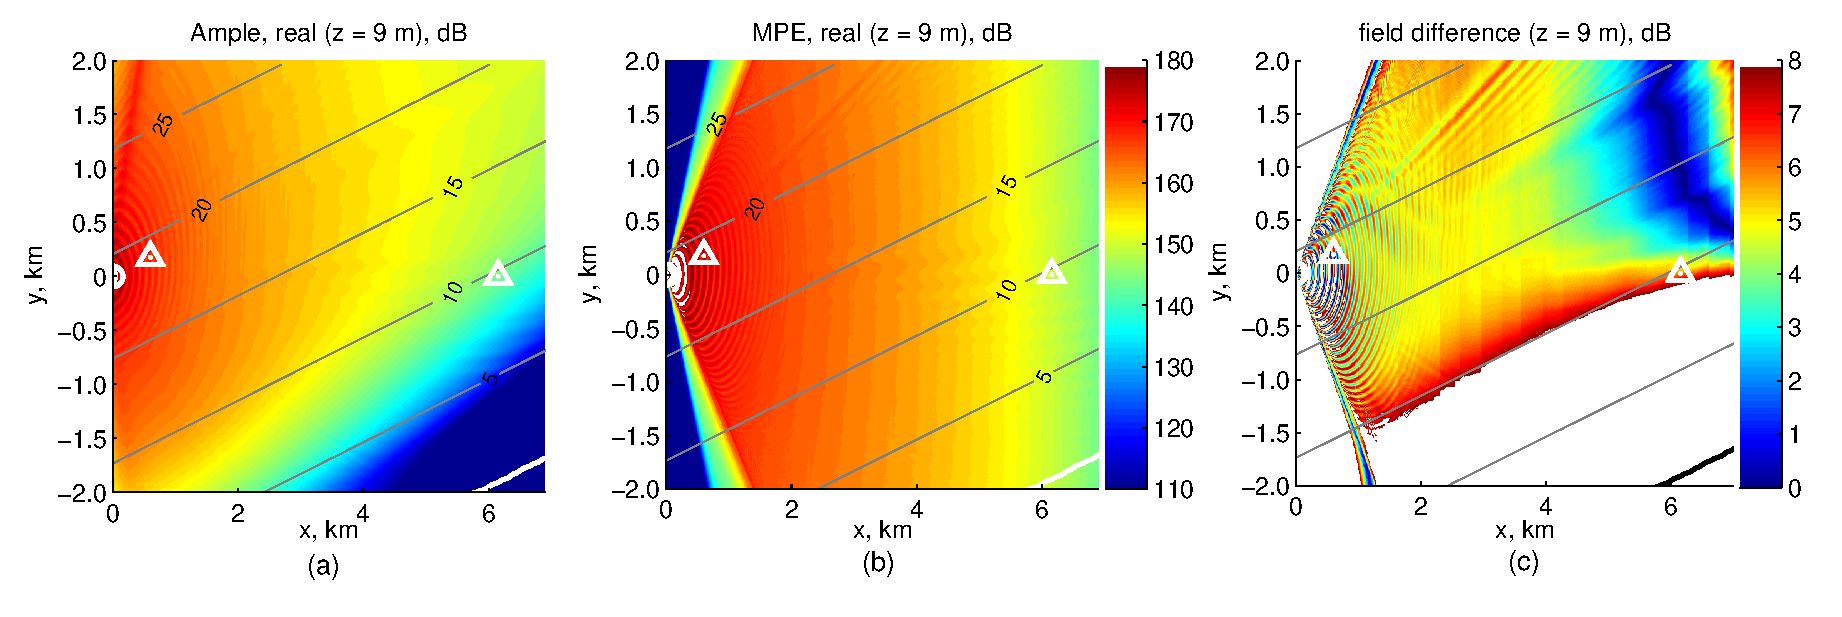
\includegraphics[width=0.95\textwidth]{seismo/pic_lineField.eps}
    			\caption{
                    \fefuchooselanguage{
                        russian={Пространственное распределение уровня звуковой экспозиции при глубине 9 м в волноводе с упрощённой батиметрией},
                        english={Spatial distribution of sound exposure level at 9 m in the simplified waveguide model}
                    }
                }
    		\end{figure}
    	\end{frame}
    }

	\begin{frame}{\fefuchooselanguage{russian={Реальная батиметрия},english={Realistic waveguide model}}}
		\begin{figure}[h]
			\centering
			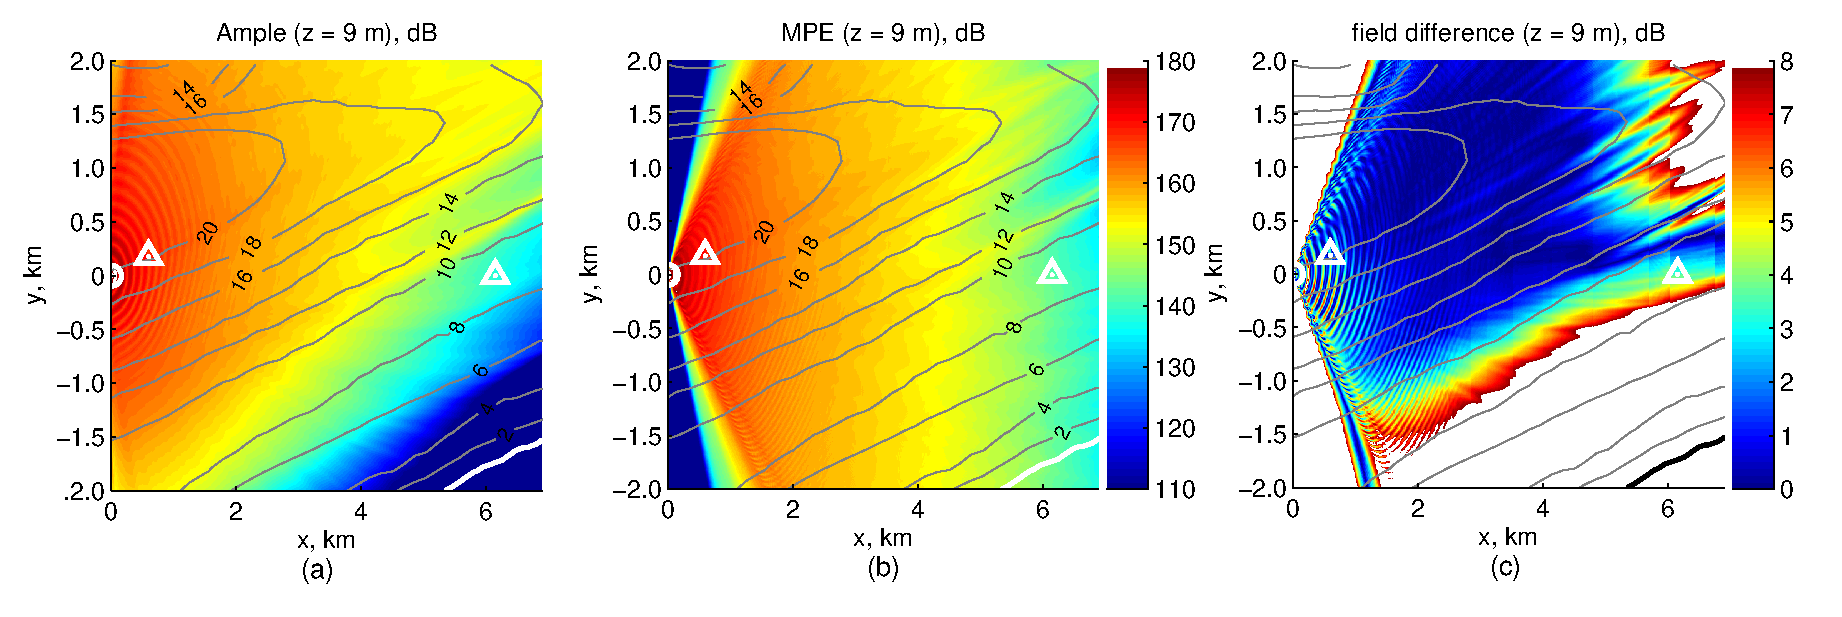
\includegraphics[width=0.95\textwidth]{seismo/pic_realField.eps}
			\caption{
                \fefuchooselanguage{
                    russian={Пространственное распределение уровня звуковой экспозиции при глубине 9 м в волноводе с реальной батиметрией},
                    english={Spatial distribution of sound exposure level at 9 m in the realistic waveguide model}
                }
            }
		\end{figure}
	\end{frame}

	\begin{frame}{\fefuchooselanguage{russian={Результаты моделирования},english={Modeling results}}}
		\begin{figure}[h]
			\centering
			\includegraphics[width=0.8\textwidth]{seismo/pic_test_sel.eps}
			\caption{
                \fefuchooselanguage{
                    russian={График зависимости уровня звуковой экспозиции от расстояния $x$ на прямой $y=0$ и глубине 9 м},
                    english={Plot of the sound exposure level as a function of distance $x$ along the line $y=0$ at a depth of 9 m}
                }
            }
		\end{figure}
	\end{frame}

	\begin{frame}{\fefuchooselanguage{russian={Результаты моделирования},english={Modeling results}}}
		\begin{figure}[h]
			\centering
			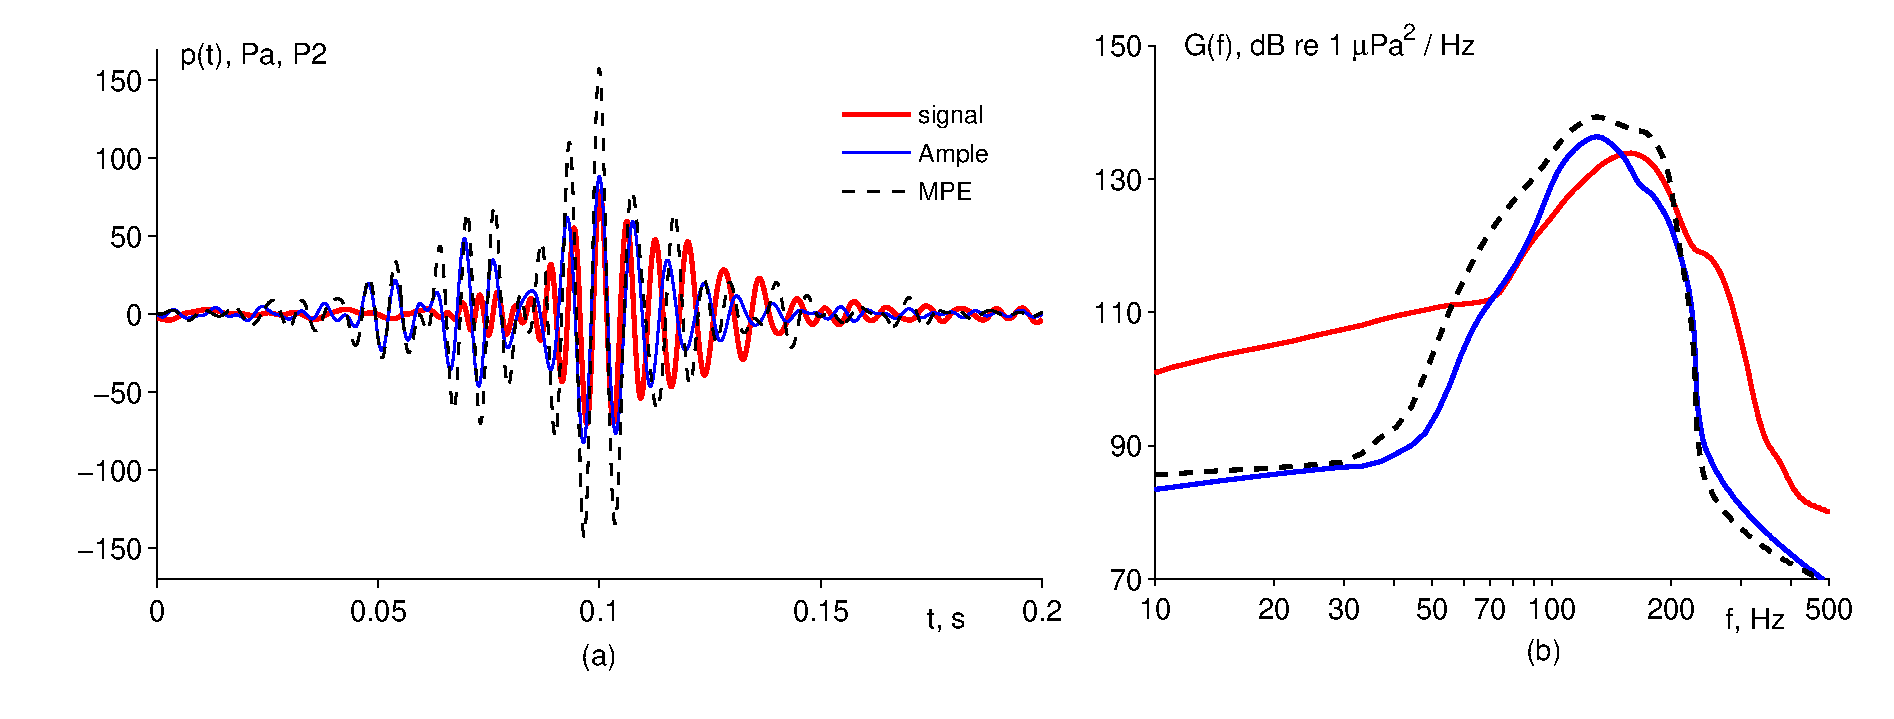
\includegraphics[width=0.9\textwidth]{seismo/pic_signal3.eps}
			\caption{
                \fefuchooselanguage{
                    russian={Сравнение импульсных сигналов (\textbf{a}) и их спектров (\textbf{b})},
                    english={Comparison of pulse signals (\textbf{a}) and their spectra (\textbf{b})}
                }
            }
		\end{figure}
	\end{frame}

	\begin{frame}{\fefuchooselanguage{russian={Выводы},english={Summary}}}
        \small
		\begin{block}{}
            \fefuchooselanguage{
                russian={Проведено моделирование акустических полей в задачах оценки уровней антропогенных шумов. Предложен способ оптимизации параметров среды и показана его эффективность. Исследована важность использования широкоугольного уравнения.},
                english={Acoustic field modeling was performed for assessing levels of anthropogenic noise. A method for optimizing environmental parameters was proposed, and its effectiveness was demonstrated. The importance of using the wide-angle equation was investigated.}
            }
		\end{block}
        \begin{block}{\fefuchooselanguage{russian={Личный вклад автора},english={Author contribution}}}
            \begin{itemize}
                \item \fefuchooselanguage{russian={Разработка метода оптимизации параметров среды на основе данных, записанных в точке ближнего прохода},english={Development of environmental parameters optimization method based on the data at the CPA}}
                \item \fefuchooselanguage{russian={Реализация алгоритма расчёта импульсов звукового сигнала и SEL на основе записи в опорной точке},english={Implementation of sound pulses and SEL computation based on the data recorded at a reference point}}
            \end{itemize}
        \end{block}
        \vspace{-0.25cm}
        \begin{block}{\fefuchooselanguage{russian={Статьи},english={Papers}}}
            \begin{refsection}
                \vspace{-0.25cm}
                \nocite{jmse,petrov2024_2}
                \AtNextBibliography{\changefontsizes{7.5pt}}
                \printbibliography[heading=none,env=betterlabel,keyword={myarticles}]
            \end{refsection}
        \end{block}
	\end{frame}

	\begin{frame}{\fefuchooselanguage{russian={Положения, выносимы на зашиту},english={Key claims to be defended}}}
		\vskip -1cm
		\begin{block}{}
			\footnotesize
			\begin{enumerate}
				\item \fefuchooselanguage{
                    russian={Разработана и апробирована методика численного решения псевдодифференциальных модовых параболических уравнений с искусственным ограничением расчётной области путём постановки граничных условий прозрачности или добавления к ней согласованных поглощающих слоёв},
                    english={A mehod for the numerical solution of pseudodifferential mode parabolic equations has been developed and tested, with the artificial truncation of the computational domain through the implementation of transparent boundary conditions or the perfectly matching layers.}
                }
				\item \fefuchooselanguage{
                    russian={Разработан комплекс программ на языке программирования C++, который может быть использован для моделирования распространения тональных и импульсных сигналов, а также вычисления скалярных и векторных акустических полей антропогенных шумов в океане с возможностью учёта батиметрических и гидрологических данных и структуры слоёв дна, и ориентированный на максимальную производительность},
                    english={A software suite has been developed in the C++ programming language, which can be used for modeling the propagation of tonal and pulse signals, as well as calculating scalar and vector acoustic fields of anthropogenic noise in the ocean. The program allows to set bathymetric and hydrological data, the structure of seabed layers and other media parameters.}
                }
				\item \fefuchooselanguage{
                    russian={Моделирование антропогенных шумов, связанных с сейсморазведочными работами и судоходством, проведённое с использованием разработанного комплекса прикладных программ, позволило добиться согласия уровней акустической экспозиции (SEL) с данными прямых измерений с точностью до 1 дБ. и согласия значений распределения энергии в децидекадных частотных полосах на различных расстояниях от источника шума с точностью до 5 дБ. для диапазона частот, в котором сосредоточена большая часть энергии сигнала},
                    english={The modeling of anthropogenic noise related to seismic survey and vessel transfer performed using the developed software achieves a good agreement of sound exposure levels with direct measurements data with an accuracy of up to 1 dB. Additionally, the software achieved agreement of energy distribution values in decidecade frequency bands at various distances from the noise source with an accuracy of up to 5 dB for the frequency range with the most energy.}
                }
			\end{enumerate}
		\end{block}
	\end{frame}

	\begin{frame}{\fefuchooselanguage{russian={Научные труды. Статьи},english={Papers}}}
		\AtNextBibliography{\changefontsizes{7.5pt}}
		\printbibliography[heading=none,env=betterlabel,keyword={myarticles}]
	\end{frame}

	\begin{frame}{\fefuchooselanguage{russian={Научные труды. Материалы конференций},english={Conference papers}}}
		\AtNextBibliography{\changefontsizes{8pt}}
		\printbibliography[heading=none,env=betterlabel,keyword={myproceedings}]
	\end{frame}

	\begin{frame}
		\thispagestyle{empty}
		\addtocounter{framenumber}{-1}
		\centerline{\Huge \fefuchooselanguage{russian={Спасибо за внимание},english={Thank you for your attention}}}
	\end{frame}

    \begin{multline}\mathbf{A}\cdot SPD+\mathbf{B}\cdot OTF^\mathbf{D}\cdot\max\left(ATK,SP.ATK\right)+\\\frac{\mathbf{C}}{DTF^\mathbf{E}}\cdot\sqrt{HP\cdot\sqrt[\mathbf{F}+\mathbf{G}]{SP.DEF^\mathbf{F}\cdot DEF^\mathbf{G}}}\end{multline}

\end{document}
